\makeatletter
\@ifundefined{captionsfrench}{%
  \PackageWarningNoLine{ch-Resume}{La langue french n'est pas chargée par
    Babel : le résumé sera composé avec les règles anglaises}%
  \providecommand{\resumeLangueDebut}{}%
  \providecommand{\resumeLangueFin}{}%
  \providecommand{\resumeTikzSafe}{}%
}{
  \providecommand{\resumeLangueDebut}{\begin{otherlanguage}{french}}
  \providecommand{\resumeLangueFin}{\end{otherlanguage}}
  \providecommand{\resumeTikzSafe}{\shorthandoff{;:!?}}
}
\makeatother

\begingroup
\resumeLangueDebut
\renewcommand{\tablename}{Tableau}

\chapter*{Résumé en français}
\markboth{RÉSUMÉ EN FRANÇAIS}{RÉSUMÉ EN FRANÇAIS}
\addcontentsline{toc}{chapter}{Résumé en français}
\label{ch:resume}

% numérotation propre au résumé : I, I.1, ...
\setcounter{section}{0}
\renewcommand{\thesection}{\Roman{section}}
\renewcommand{\thesubsection}{\thesection.\arabic{subsection}}
\counterwithin*{figure}{section}
\counterwithin*{table}{section}
\counterwithin*{equation}{section}
\setcounter{figure}{0}\setcounter{table}{0}\setcounter{equation}{0}
\renewcommand{\thefigure}{\thesection.\arabic{figure}}
\renewcommand{\thetable}{\thesection.\arabic{table}}
\renewcommand{\theequation}{\thesection.\arabic{equation}}
\renewcommand{\theHsection}{resume.\Roman{section}}
\renewcommand{\theHfigure}{resume.\Roman{section}.\arabic{figure}}
\renewcommand{\theHtable}{resume.\Roman{section}.\arabic{table}}
\renewcommand{\theHequation}{resume.\Roman{section}.\arabic{equation}}

Ma thèse, intitulée «~Recherche de nouvelles particules à long temps de vie et fortement ionisantes avec l'expérience CMS~», a été préparée au sein du groupe CMS de l'Institut Pluridisciplinaire Hubert Curien (IPHC) de Strasbourg, sous la direction de Caroline Collard. Elle porte sur la recherche de particules lourdes, chargées et stables à l'échelle du détecteur (\textit{Heavy Stable Charged Particles}, HSCP) dans les collisions proton--proton enregistrées par l'expérience CMS (\textit{Compact Muon Solenoid}) au LHC (\textit{Large Hadron Collider}) pendant le Run--3. Ce résumé reprend l'ensemble des chapitres du manuscrit, rédigé en anglais, dans le même ordre.


%% ---------------------------------------------------------------------
\section*{Introduction}
\addcontentsline{toc}{section}{Introduction}
\label{sec:resume:intro}

Le Modèle Standard (MS) de la physique des particules décrit les constituants élémentaires de la matière et trois des quatre interactions fondamentales, dans le cadre de la théorie quantique des champs et de l'invariance de jauge locale. Ses prédictions ont été confirmées avec une grande précision par plusieurs générations d'expériences, et la découverte du boson de Higgs par les collaborations ATLAS et CMS en 2012~\cite{ATLAS_Higgs, CMS_Higgs} a complété sa description en termes de particules. Le MS laisse pourtant plusieurs questions ouvertes : il ne contient aucun candidat à la matière noire, n'explique pas l'asymétrie entre matière et antimatière observée dans l'Univers et n'inclut pas la gravitation. Il est donc vraisemblablement la limite à basse énergie d'une théorie plus complète, ce qui motive la recherche directe de nouvelle physique au LHC.

Parmi les signatures possibles, les particules à long temps de vie (\textit{long-lived particles}, LLP) occupent une place particulière. La plupart des recherches de LLP ciblent des états neutres qui se désintègrent dans le volume du détecteur. Cette thèse s'intéresse au cas opposé : des particules chargées, massives (de quelques centaines de GeV à quelques TeV) et suffisamment stables pour traverser l'intégralité du détecteur CMS. Produites à faible vitesse, ces HSCP laissent une trace de forte impulsion, associée à une perte d'énergie par ionisation (\dedx) anormalement élevée, une signature pratiquement absente des processus du MS.

Le manuscrit comporte quatre chapitres. Le premier présente le LHC, le détecteur CMS et les méthodes de reconstruction des événements. Le deuxième porte sur la mesure de la charge déposée dans le trajectographe à pistes de silicium et sur le développement d'une nouvelle correction de la saturation de l'électronique de lecture, qui biaise la mesure de \dedx{} pour les dépôts fortement ionisants. Le troisième rappelle le cadre théorique et le contexte expérimental des recherches de HSCP. Le quatrième détaille la recherche de HSCP menée avec les données enregistrées en 2024 à une énergie dans le centre de masse $\sqrt{s}=13{,}6$~TeV, interprétée dans le cadre de la production de paires de gluinos formant des $R$-hadrons.


%% ---------------------------------------------------------------------
\section{L'expérience CMS au LHC}
\label{sec:resume:cms}

\subsection{Le Grand collisionneur de hadrons}

Le LHC~\cite{EvansBryant2008}, installé à environ 100~m sous la frontière franco-suisse dans un tunnel de 26,7~km de circonférence, est le plus grand accélérateur de particules jamais construit. Les protons, préaccélérés jusqu'à 450~GeV par une chaîne d'injecteurs, y sont portés à 6,8~TeV, tandis que 1 232 dipôles supraconducteurs, refroidis à 1,9~K, les maintiennent sur leur orbite avec un champ de 8,1~T. Les deux faisceaux circulent en sens opposés sous forme de paquets espacés de 25~ns et se croisent en quatre points d'interaction, où sont installées les expériences ATLAS, CMS, LHCb et ALICE.

La luminosité instantanée $\mathscr{L}$ mesure la capacité du collisionneur à produire des interactions. Elle relie le taux d'événements d'un processus à sa section efficace $\sigma$, $\mathrm{d}N/\mathrm{d}t=\mathscr{L}\cdot\sigma$, et ne dépend que des paramètres des faisceaux : nombre de protons par paquet, nombre de paquets, fréquence de révolution et taille des faisceaux au point d'interaction. Intégrée sur la durée de prise de données, elle donne la luminosité intégrée, exprimée en fb$^{-1}$, qui détermine le nombre d'événements produits : $\displaystyle N=\sigma\cdot\int\mathscr{L}\,\mathrm{d}t$. Augmenter la luminosité instantanée accroît également l'empilement (\textit{pile-up}), c'est-à-dire le nombre de collisions simultanées lors du croisement de paquets. Depuis 2024, l'empilement atteint en moyenne une soixantaine d'interactions. À la suite du Run--1 ($\sqrt{s}=7$ et 8~TeV, environ 30~fb$^{-1}$ enregistrés) et du Run--2 ($\sqrt{s}=13$~TeV, environ 138~fb$^{-1}$ enregistrés), le Run--3 a augmenté l'énergie de centre de masse à 13,6~TeV. Au cours de cette période (2022--2026), CMS a collecté environ 310~fb$^{-1}$ de données validées. Le LHC à haute luminosité (HL-LHC), qui lui succédera après le troisième long arrêt, doit délivrer 3 000 à 4 000~fb$^{-1}$ avec un empilement pouvant atteindre 200 interactions par croisement.


\subsection{Le détecteur CMS}

CMS~\cite{CMS_detector} est un détecteur généraliste cylindrique, long de 21~m et d’un diamètre de 15~m. Ses sous-détecteurs sont disposés en couches concentriques autour de l'axe des faisceaux, dans une partie centrale (le tonneau) fermée par deux bouchons. Un solénoïde supraconducteur produit un champ magnétique de 3,8~T parallèle aux faisceaux, qui courbe la trajectoire des particules chargées et permet de mesurer leur impulsion. Les directions sont identifiées par l'angle azimutal $\phi$ et la pseudo-rapidité $\eta=-\ln[\tan(\theta/2)]$, où $\theta$ est l'angle polaire.

Le trajectographe au silicium, le plus proche du point d'interaction, couvre la région $|\eta|<2{,}5$ (\hyperref[fig:resume:tracker]{Figure~\ref*{fig:resume:tracker}}). Le détecteur à pixels comprend quatre couches dans le tonneau et trois disques dans chaque bouchon ; la finesse de ses cellules ($100\times150~\mu$m$^2$) permet de reconstruire les vertex primaires et secondaires. Il est entouré du trajectographe à pistes : quatre couches internes (TIB) et six couches externes (TOB) dans le tonneau, trois disques internes (TID) et neuf disques externes (TEC) dans chaque bouchon, soit 15\,148 modules. Les capteurs ont une épaisseur de 320 ou 500~$\mu$m et un pas inter-pistes compris entre 80 et 205~$\mu$m. Outre la position des impacts, les modules à pistes mesurent la charge collectée, ce qui permet d'accéder à la perte d'énergie par unité de longueur \dedx{}, au cœur de la recherche de HSCP.

\begin{figure}[h!]
    \centering
    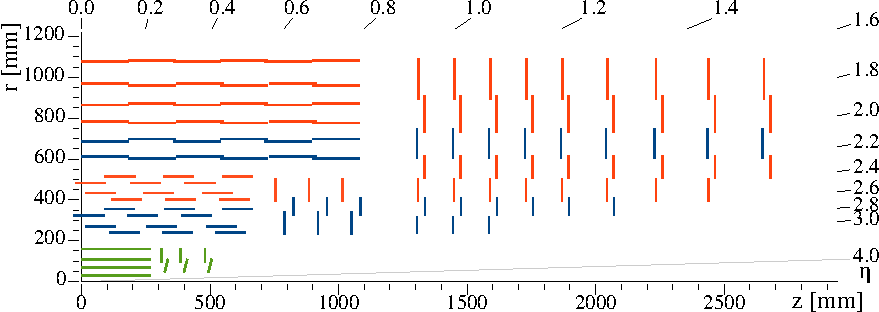
\includegraphics[width=0.95\linewidth]{Images/Ch1/Phase1_Tracker_1Quarter.pdf}
    \caption{Coupe longitudinale d'un quart du trajectographe de CMS dans le plan $r$--$z$. Les modules à pixels sont représentés en vert, les modules à pistes simple face et double face en rouge et en bleu.}
    \label{fig:resume:tracker}
\end{figure}

Autour du trajectographe, le calorimètre électromagnétique (ECAL), constitué de cristaux scintillants de tungstate de plomb, et le calorimètre hadronique (HCAL), qui alterne des absorbeurs en laiton et des scintillateurs, mesurent l'énergie des électrons, des photons et des hadrons. Le système à muons, logé dans le retour de flux de l'aimant, combine des tubes à dérive, des chambres à pistes cathodiques et des chambres à plaques résistives.

\subsection{Déclenchement et reconstruction des événements}

Les croisements de paquets ont lieu à 40~MHz. Un premier niveau de déclenchement matériel (L1), fondé sur les calorimètres et les chambres à muons, réduit ce taux à 100~kHz en 3,8~$\mu$s ; le système de déclenchement de haut niveau (HLT), logiciel, le ramène ensuite à environ 2,6~kHz. J'ai contribué à la surveillance de ce système lors de 27 gardes (\textit{shifts}) de huit heures pendant le Run--3.

La reconstruction repose sur l'algorithme de flux de particules (\textit{Particle Flow}, PF)~\cite{PFalgo}, qui combine les informations de tous les sous-détecteurs pour identifier les muons, les électrons, les photons et les hadrons, chargés comme neutres. Les traces, reconstruites itérativement à l'aide d'un filtre de Kalman, sont classées par qualité, la plus stricte étant \textit{HighPurity}. Deux variables d'isolation sont utilisées dans l'analyse : $I_\mathrm{rel}^\mathrm{PF}$, somme des impulsions transverses des candidats PF dans un cône $\Delta R$ variable autour de la trace, normalisée à celle de la trace, et $I_\mathrm{trk}$, somme des impulsions transverses des autres traces dans un cône $\Delta R<0{,}3$. Les jets sont formés par l'algorithme anti-$k_t$ ($R=0{,}4$), après pondération des candidats selon la méthode PUppi, qui réduit l'effet de l'empilement.

L'énergie transverse manquante (MET), la norme de l'opposé de la somme vectorielle des impulsions transverses reconstruites, joue un rôle central dans cette thèse. La MET PF, ou sa variante MET PUppi, est construite à partir de tous les candidats PF, tandis que la MET calorimétrique (Calo MET) n'utilise que les dépôts dans les calorimètres. Une particule qui traverse les calorimètres en y déposant peu d'énergie, comme un muon ou une HSCP, est donc invisible pour la Calo MET mais prise en compte dans la MET PF. On définit aussi $H_\mathrm{T}$, somme scalaire des impulsions transverses des jets, et MHT, norme de leur somme vectorielle (MHT$^\mathrm{NoMu}$ lorsque les muons sont exclus). Enfin, les simulations Monte-Carlo (MC) enchaînent la génération du processus dur, le développement des gerbes partoniques et l'hadronisation, puis la réponse du détecteur (\textsc{Geant4}), avant une reconstruction identique à celle des données.


%% ---------------------------------------------------------------------
\section[Reconstruction de la charge des particules ionisantes]{Reconstruction de la charge des particules ionisantes dans le trajectographe}
\label{sec:resume:saturation}

\subsection{Perte d'énergie par ionisation}

Une particule chargée traversant la matière perd de l'énergie principalement par ionisation. La perte d'énergie moyenne est décrite par la formule de Bethe-Bloch~\cite{PDG}, qui ne dépend de la particule que par sa charge et le produit $\beta\gamma=p/M$ : elle décroît comme $1/\beta^2$ à basse vitesse, atteint un minimum autour de $\beta\gamma\approx3$--4, puis remonte lentement dans le régime relativiste. La grande majorité des particules reconstruites dans CMS se situe près de ce minimum ; on les qualifie de particules au minimum d'ionisation (MIP). À impulsion donnée, une particule plus lourde présente un $\beta\gamma$ plus faible et dépose donc davantage d'énergie : la mesure simultanée de $p$ et de \dedx{} permet d'estimer sa masse.

Dans une couche mince de silicium, la charge déposée fluctue fortement d'un module à l'autre, en raison de transferts d'énergie rares mais importants aux électrons du milieu (rayons $\delta$) : elle suit une distribution de Landau~\cite{Landau} asymétrique, que l'on caractérise par sa valeur la plus probable (MPV).

\subsection{Les modules à pistes de silicium}

Les capteurs du trajectographe sont des jonctions p--n : des pistes implantées p$^+$ sur un substrat de type n, polarisées en inverse pour être entièrement déplétées. Une MIP y crée environ 70 paires électron-trou par micromètre. Le signal induit sur les pistes est mis en forme par les puces APV25, qui lisent chacune 128 pistes, puis transmis par fibre optique aux cartes FED, qui le numérisent sur 10~bits, soustraient le piédestal et le bruit de mode commun.

Avant stockage, l'amplitude est réduite de 10 à 8~bits : les pistes en dessous de 254 coups ADC sont conservées telles quelles, celles comprises entre 254 et 1022 coups sont fixées à 254, et celles au-delà de 1023 coups à 255. Les pistes adjacentes sont ensuite regroupées en amas (\textit{clusters}). Deux effets élargissent un amas : le partage de charge, lorsque la particule traverse le capteur à un angle d'incidence élevé, et la diaphonie capacitive (\textit{cross-talk}) entre pistes voisines. Cette dernière redistribue une fraction connue de la charge de la piste centrale vers ses voisines immédiates ($x_1$) et ses secondes voisines ($x_2$), avec $x_0+2x_1+2x_2=1$ ; une particule d'incidence quasi perpendiculaire au module produit ainsi un amas symétrique en forme de pyramide. Les paramètres de diaphonie, mesurés en 2010 puis en 2018~\cite{Xtalk2018CMS}, diminuent avec l'âge des capteurs.

\subsection{L'estimateur \texorpdfstring{$I_h$}{Ih} et la saturation des amas}

La perte d'énergie moyenne le long d'une trace est estimée par la moyenne harmonique d'ordre $-2$ des $N$ mesures $c_j=(\dedx)_j$ qui lui sont associées :
\begin{equation}
    I_h=\left(\frac{1}{N}\sum_{j=1}^{N}c_j^{-2}\right)^{-1/2} .
    \label{eq:resume:ih}
\end{equation}
Cet estimateur est peu sensible aux fortes fluctuations de la queue de Landau, mais très sensible aux sous-estimations. La saturation biaise la valeur de $I_h$ : une fois le plafond de 8~bits atteint, l'amplitude enregistrée ne contient plus d'information sur la charge réelle. Un amas contenant au moins une piste à 254 ou 255 coups ADC est dit saturé.

Pour étudier cet effet, j'ai utilisé un échantillon simulé de muons émis dos à dos (MC--muon) dans lequel la charge simulée avant saturation est conservée, des échantillons simulés $W$+jets et de gluinos de 2000~GeV, ainsi que des données de 2018. Sur des traces de bonne qualité, la fraction d'amas saturés est de 8,8\,\% dans MC--muon et de 8,9\,\% dans les données, mais atteint 44\,\% pour les gluinos. Parmi les amas saturés, dans tous les échantillons, on observe qu'une seule piste est saturée dans 86 à 94\,\% des cas, et deux pistes consécutives dans 5 à 9\,\% des cas. La charge reconstruite des amas saturés est systématiquement inférieure à la charge vraie (\hyperref[fig:resume:saturation]{Figure~\ref*{fig:resume:saturation}}), et ce biais se propage directement à $I_h$.

\begin{figure}[h!]
    \centering
    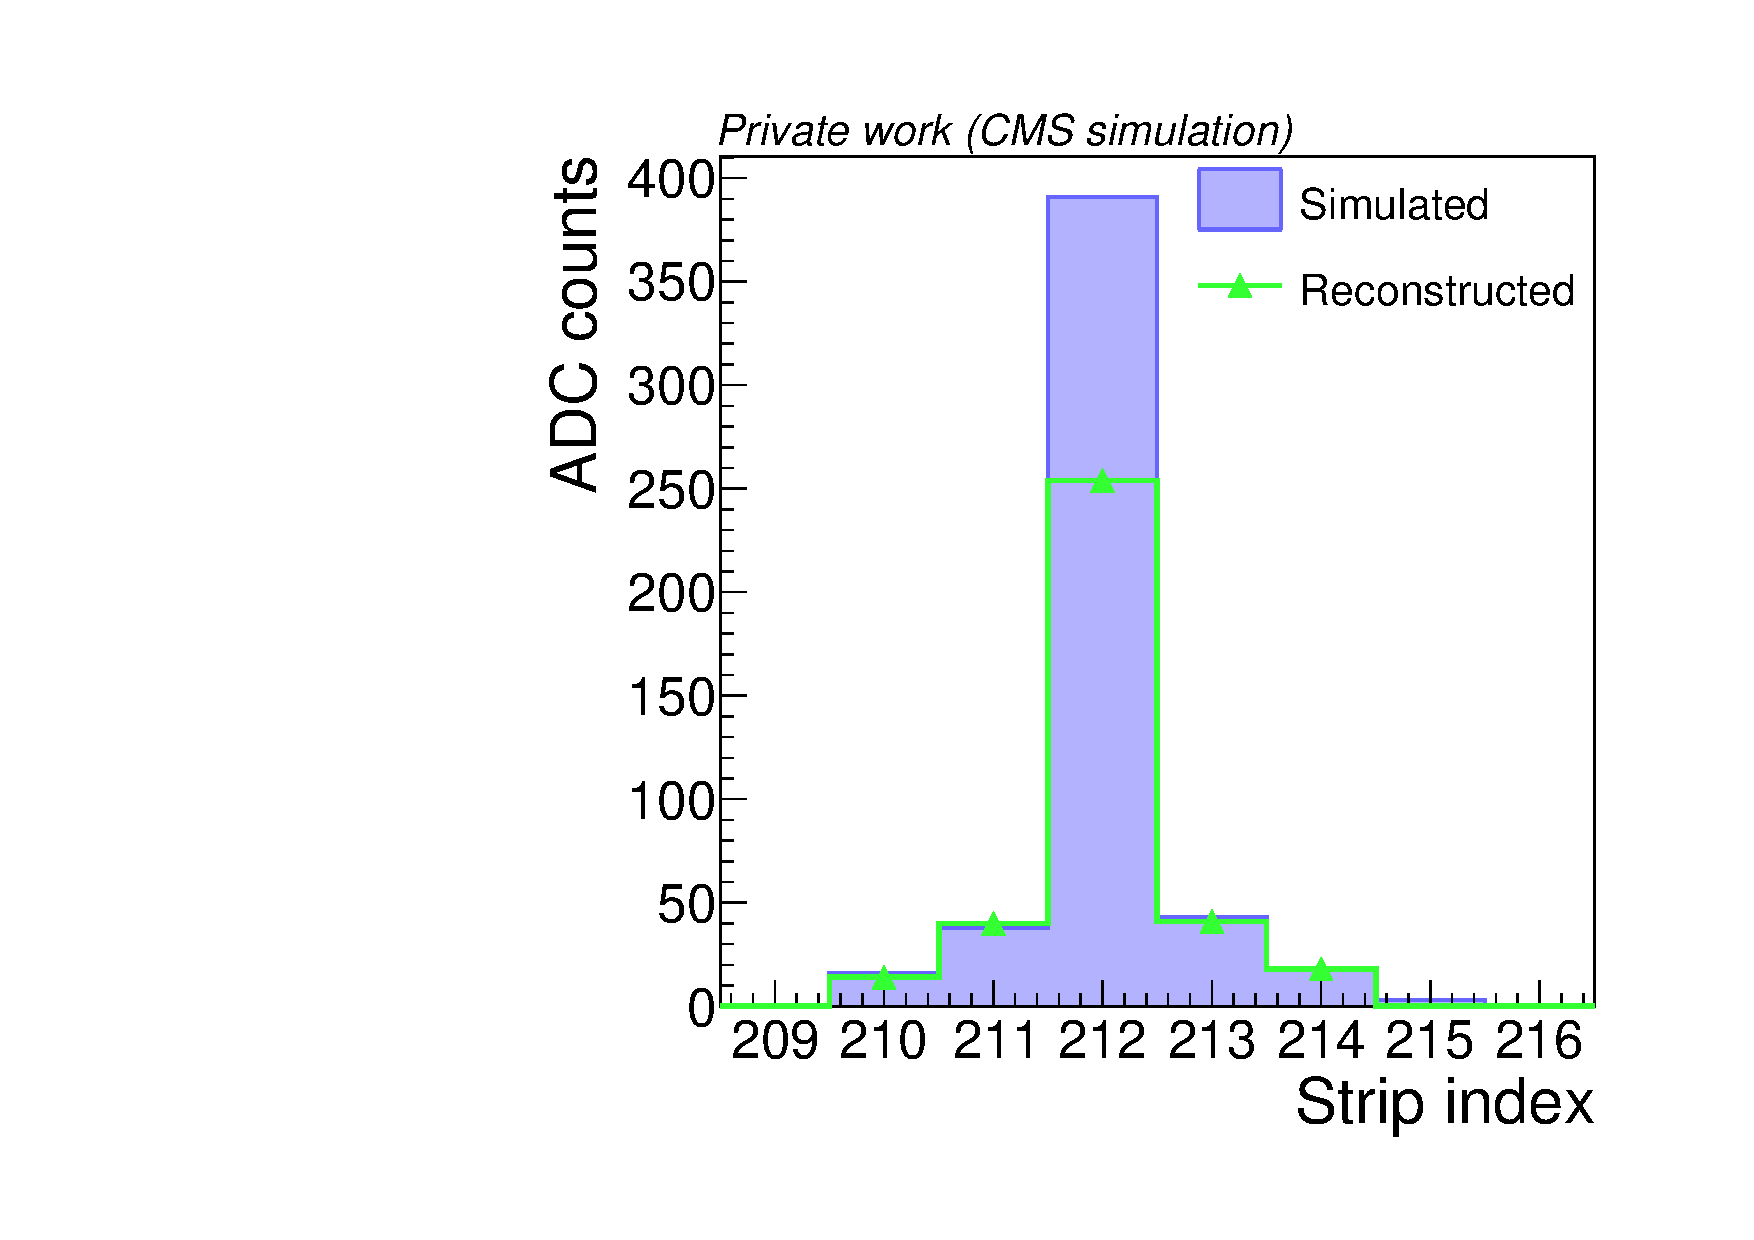
\includegraphics[width=0.48\linewidth,trim={0.3cm 0.8cm 2cm 0.8cm},clip,valign=c]{Images/Ch2/Cluster_saturation_bis.pdf}
    \hfill
    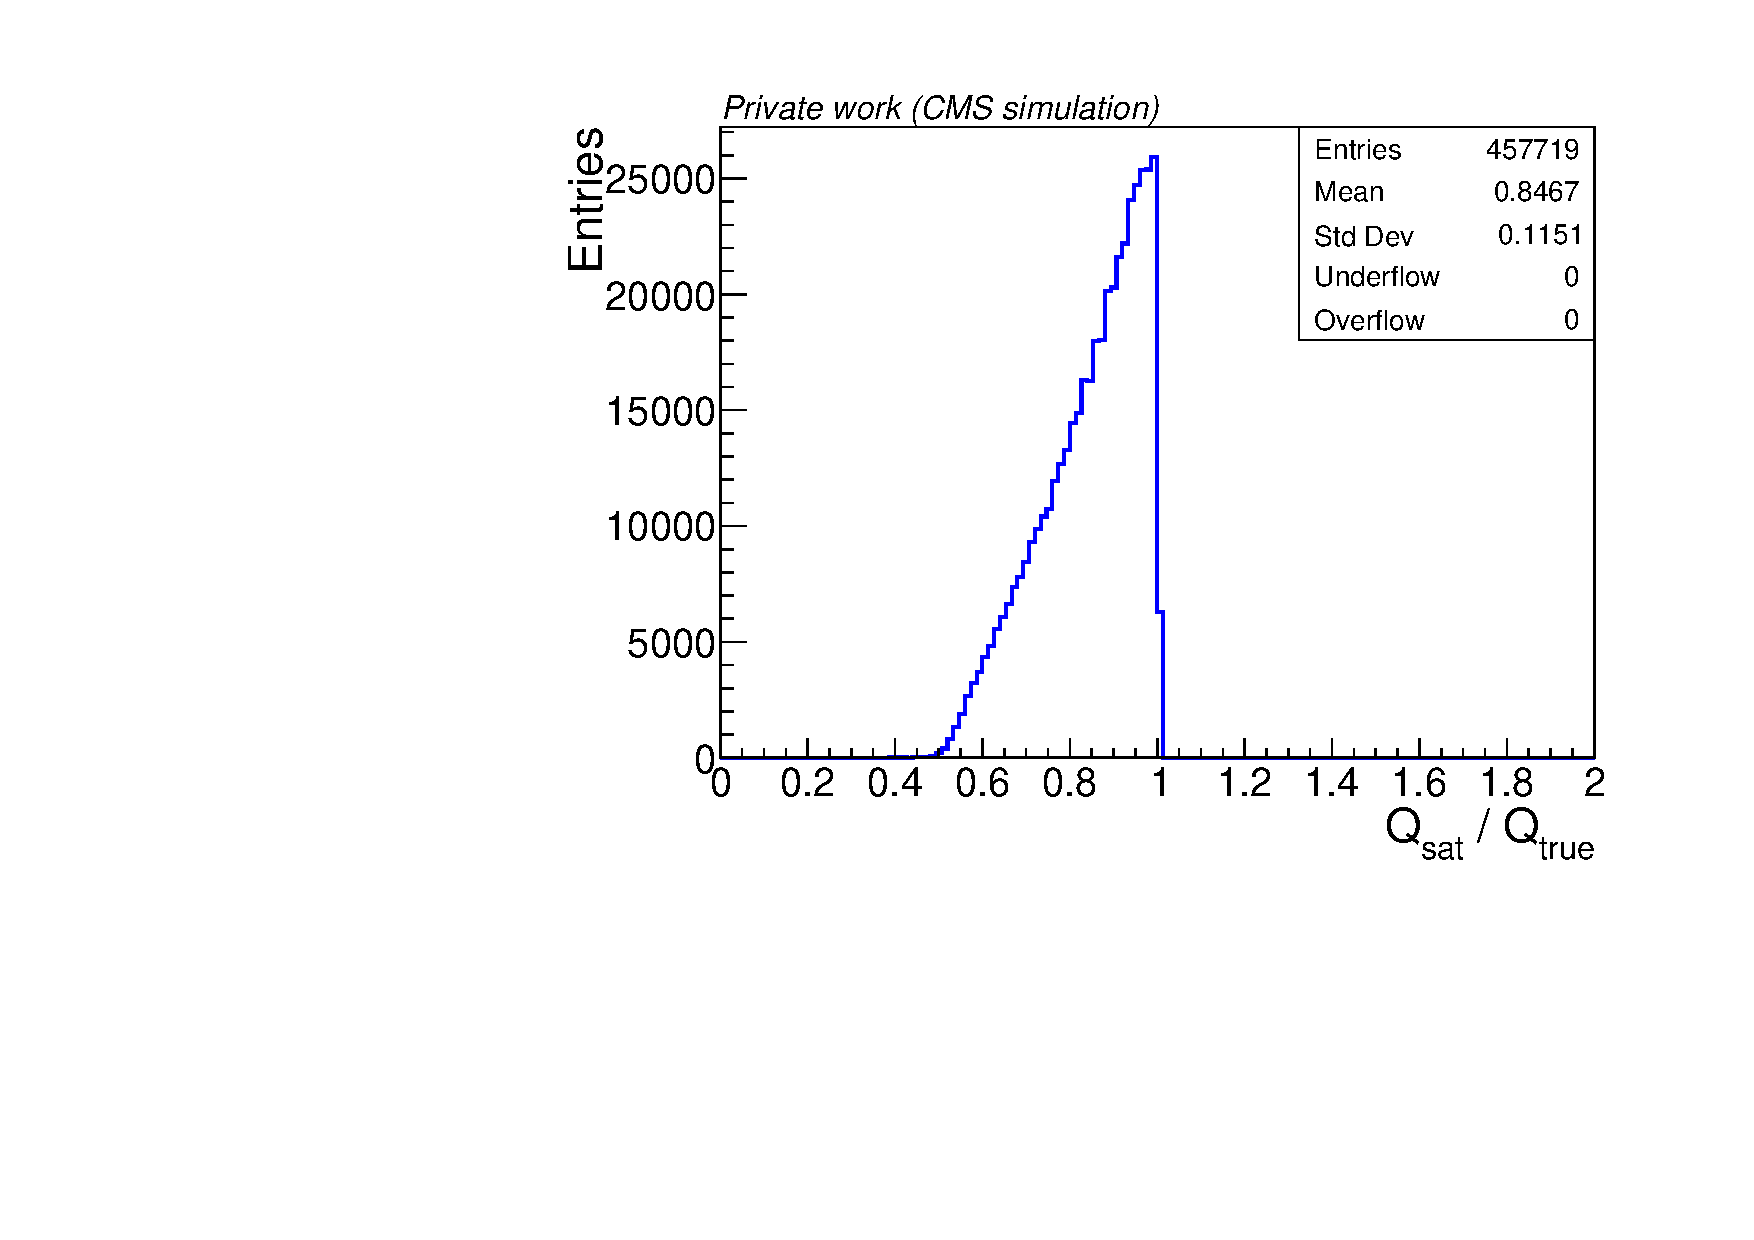
\includegraphics[width=0.48\linewidth,trim={0.5cm 0.5cm 1.8cm 0.8cm},clip,valign=c]{Images/Ch2/Qsat_VS_Qtrue_bis.pdf}
    \caption{À gauche : exemple d'amas de l'échantillon MC--muon, comparant la charge simulée (bleu) et la charge reconstruite après saturation (vert). À droite : rapport entre la charge reconstruite $Q_\mathrm{sat}$ et la charge vraie $Q_\mathrm{true}$ des amas saturés de MC--muon.}
    \label{fig:resume:saturation}
\end{figure}

\subsection{La correction de base et ses limites}

La correction utilisée par les analyses HSCP depuis le Run--1~\cite{CMS_HSCP_7TeV, HSCP_Run2} inverse la diaphonie : la charge de l'amas saturé est estimée par $(L_\mathrm{max}+R_\mathrm{max})/(2x_1)$ avec $x_1=0{,}1$, où $L_\mathrm{max}$ et $R_\mathrm{max}$ sont les charges des deux pistes adjacentes au maximum. Cette correction ne s'applique qu'aux amas de 2 à 8 pistes comportant une seule piste saturée et des voisines symétriques ($|L_\mathrm{max}-R_\mathrm{max}|<40$ coups ADC, chacune au-dessus de 25 coups ADC). Sur l'échantillon MC--muon, elle sous-estime la charge d'environ 13\,\%, avec une dispersion relative du même ordre, et seuls deux tiers des amas saturés sont corrigés. La dispersion provient du coefficient $x_1$ constant, tandis que la diaphonie dépend de la géométrie des capteurs ; la faible fraction d'amas corrigés s'explique par des critères de sélection restrictifs et par l'absence de traitement des amas à deux pistes saturées.

\subsection{Une correction fondée sur la forme des amas}

J'ai développé une nouvelle correction qui adapte l'inversion de la diaphonie en fonction de la forme de l'amas et de la région du trajectographe. Les amas comportant une seule piste saturée sont classés en cinq catégories (\hyperref[fig:resume:formes]{Figure~\ref*{fig:resume:formes}}) : \textit{Center} (69\,\% des amas saturés de MC--muon), pour lesquels les deux voisines du maximum diffèrent de moins de 10\,\% ; \textit{Left} et \textit{Right} (14\,\% chacune), produits par des traces plus inclinées, dont l'une des voisines porte nettement plus de charge ; \textit{FullLeft} et \textit{FullRight} (1,5\,\% chacune), dont le maximum se trouve au bord de l'amas, le plus souvent à cause d'une piste morte adjacente.

\begin{figure}[h!]
    \centering
    {\resumeTikzSafe
    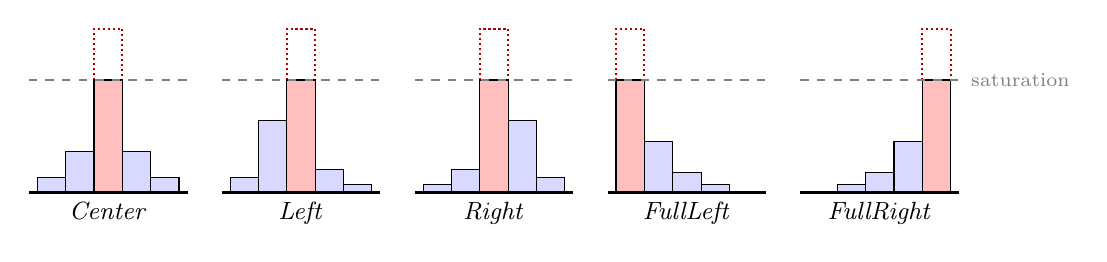
\begin{tikzpicture}[x=0.36cm, y=0.65cm, font=\small]
        % #1 : décalage horizontal, #2 : barres i/h, #3 : indice de la piste saturée, #4 : nom
        \def\amas#1#2#3#4{%
            \begin{scope}[xshift=#1 cm]
                \foreach \i/\h in {#2}{%
                    \draw[fill=blue!15] (\i,0) rectangle (\i+1,\h);
                }
                \draw[densely dotted, thick, red!70!black] (#3,2.2) -- (#3,3.2) -- (#3+1,3.2) -- (#3+1,2.2);
                \draw[fill=red!25] (#3,0) rectangle (#3+1,2.2);
                \draw[thick] (-0.3,0) -- (5.3,0);
                \draw[dashed, gray] (-0.3,2.2) -- (5.3,2.2);
                \node[below] at (2.5,0) {\textit{#4}};
            \end{scope}}
        \amas{0}{0/0.3,1/0.8,3/0.8,4/0.3}{2}{Center}
        \amas{2.45}{0/0.3,1/1.4,3/0.45,4/0.15}{2}{Left}
        \amas{4.9}{0/0.15,1/0.45,3/1.4,4/0.3}{2}{Right}
        \amas{7.35}{1/1.0,2/0.4,3/0.15}{0}{FullLeft}
        \amas{9.8}{1/0.15,2/0.4,3/1.0}{4}{FullRight}
        \node[gray, anchor=west, font=\scriptsize] at (32.6,2.2) {saturation};
    \end{tikzpicture}}
    \caption{Classification des amas comportant une seule piste saturée (en rouge). La ligne tiretée indique le seuil de saturation et la ligne pointillée la charge perdue. Les schémas sont à titre illustratif : le nombre de pistes par amas peut varier.}
    \label{fig:resume:formes}
\end{figure}

Pour chaque catégorie, la charge $S_\mathrm{max}$ de la piste saturée est reconstruite par
\begin{align}
    \textit{Center} :\quad & S_\mathrm{max}=a_\mathrm{center}\cdot \frac{L_\mathrm{max}+R_\mathrm{max}}{2} \, , \\
    \textit{Left}\,\,\textrm{et}\,\, \textit{Right} :\quad & S_\mathrm{max}=a_\mathrm{LR} \cdot N_\mathrm{max}+b_\mathrm{LR} \cdot N_\mathrm{min} \, , \\
    \textit{FullLeft}\,\,\textrm{et}\,\, \textit{FullRight} :\quad & S_\mathrm{max}=a_\mathrm{FL\text{-}FR} \cdot N_\mathrm{max} \, ,
\end{align}
où $N_\mathrm{max}$ et $N_\mathrm{min}$ désignent la plus grande et la plus petite des charges voisines du maximum. Les coefficients sont extraits de gabarits (\textit{templates}) construits à partir de l'échantillon MC--muon, dans lequel la charge vraie est connue, pour chaque couche du tonneau et chaque anneau des bouchons. Le coefficient $a_\mathrm{center}$, moyenne d'un ajustement gaussien du rapport $S_\mathrm{max}/[(L_\mathrm{max}+R_\mathrm{max})/2]$, varie de 7,5 dans les couches externes du TOB à 18,5 dans le TEC : il est plus élevé pour les capteurs de 320~$\mu$m, dans lesquels la charge s'étale moins latéralement. Pour les amas \textit{Left} et \textit{Right}, les coefficients proviennent d'un ajustement en deux étapes de $S_\mathrm{max}/N_\mathrm{max}$ en fonction de $N_\mathrm{max}/N_\mathrm{min}$, la première étape écartant 10 à 15\,\% d'amas atypiques. Le coefficient $b_\mathrm{LR}$ (entre 7,7 et 18,6) domine largement $a_\mathrm{LR}$ (entre $-0{,}23$ et $0{,}02$) : l'essentiel de la charge est reconstruit à partir de la voisine la moins chargée. Pour les amas \textit{FullLeft} et \textit{FullRight}, trop peu nombreux pour permettre un ajustement, le coefficient $a_\mathrm{FL\text{-}FR}$ (entre 7,5 et 18,3) est fixé au maximum de la distribution de $S_\mathrm{max}/N_\mathrm{max}$, les deux catégories étant regroupées. Enfin, pour les amas à deux pistes saturées consécutives, dont la forme ne peut plus être déterminée, la charge est estimée à partir des deux pistes voisines extérieures avec un coefficient unique $a_\mathrm{2strips}\approx16{,}3$. Si la charge corrigée reste inférieure au seuil de saturation, l'amas n'est pas modifié. Le code de la correction est publié sous licence libre~\cite{ShapeCorrGit}.

\subsection{Validation}

La validation principale utilise des muons issus de désintégrations de bosons $W$, sélectionnés dans les données de 2018 et dans la simulation $W$+jets. Des amas dont le maximum vrai est compris entre 240 et 250 coups ADC sont artificiellement saturés à 240 coups ADC, puis corrigés : la charge vraie étant connue, les deux méthodes peuvent être comparées directement (\hyperref[fig:resume:validation]{Figure~\ref*{fig:resume:validation}} et \hyperref[tab:resume:correction]{Tableau~\ref*{tab:resume:correction}}). Ma méthode permet de corriger 94\,\% des amas saturés avec une charge compatible avec la charge vraie à $1\sigma$ près (\hyperref[fig:resume:validation]{Figure~\ref*{fig:resume:validation}} à droite), alors que la correction de base donne une distribution nettement biaisée (\hyperref[fig:resume:validation]{Figure~\ref*{fig:resume:validation}} à gauche). La correction par forme supprime le biais (rapport moyen de 0,99 dans les données, contre 0,92 pour la correction de base) et fait passer la fraction d'amas corrigés d'environ 73\,\% à 94\,\%. Un désaccord résiduel entre les données et la simulation subsiste, car les coefficients ajustés sur MC--muon ne reproduisent pas parfaitement l'empilement et le bruit.

\begin{figure}[h!]
    \centering
    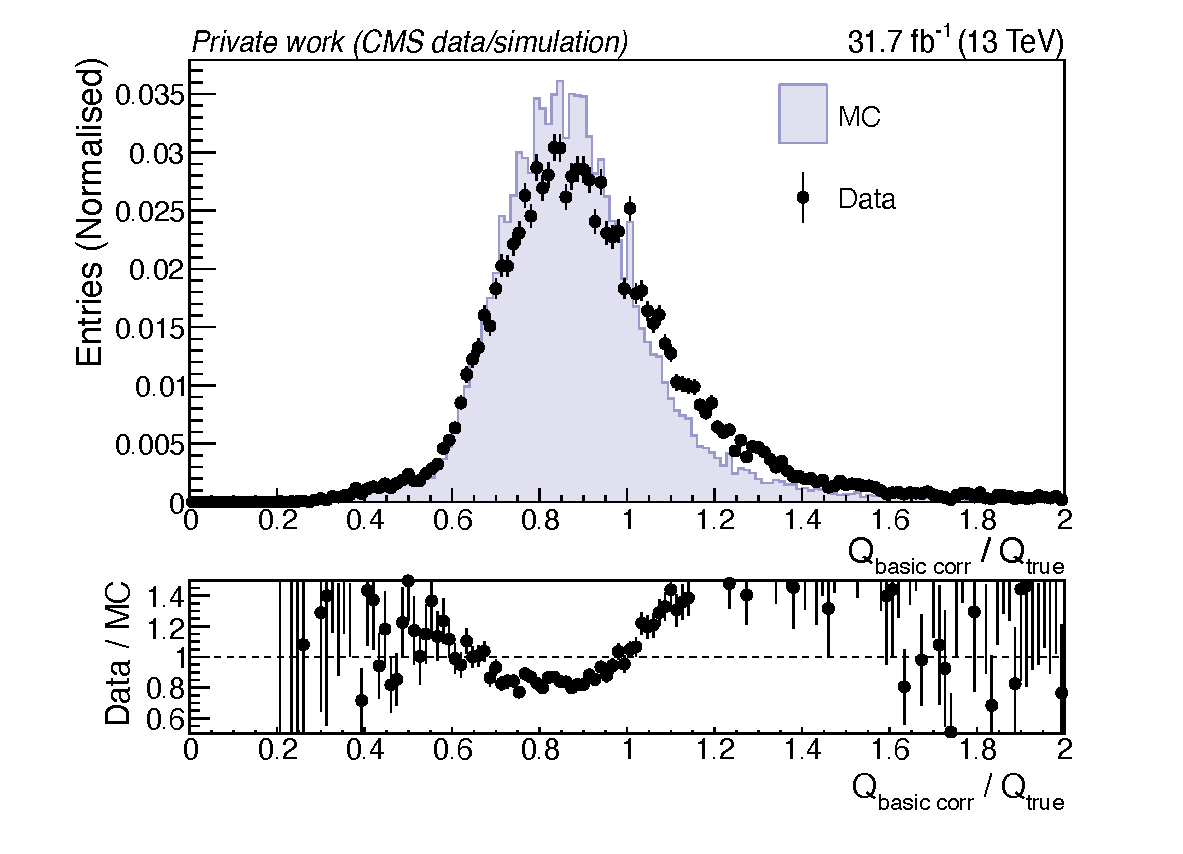
\includegraphics[width=0.49\linewidth,trim={0.8cm 0.5cm 1.5cm 0},clip]{Images/Ch2/OldCorr_dataVSmc_Wjets_weighted_bis.pdf}
    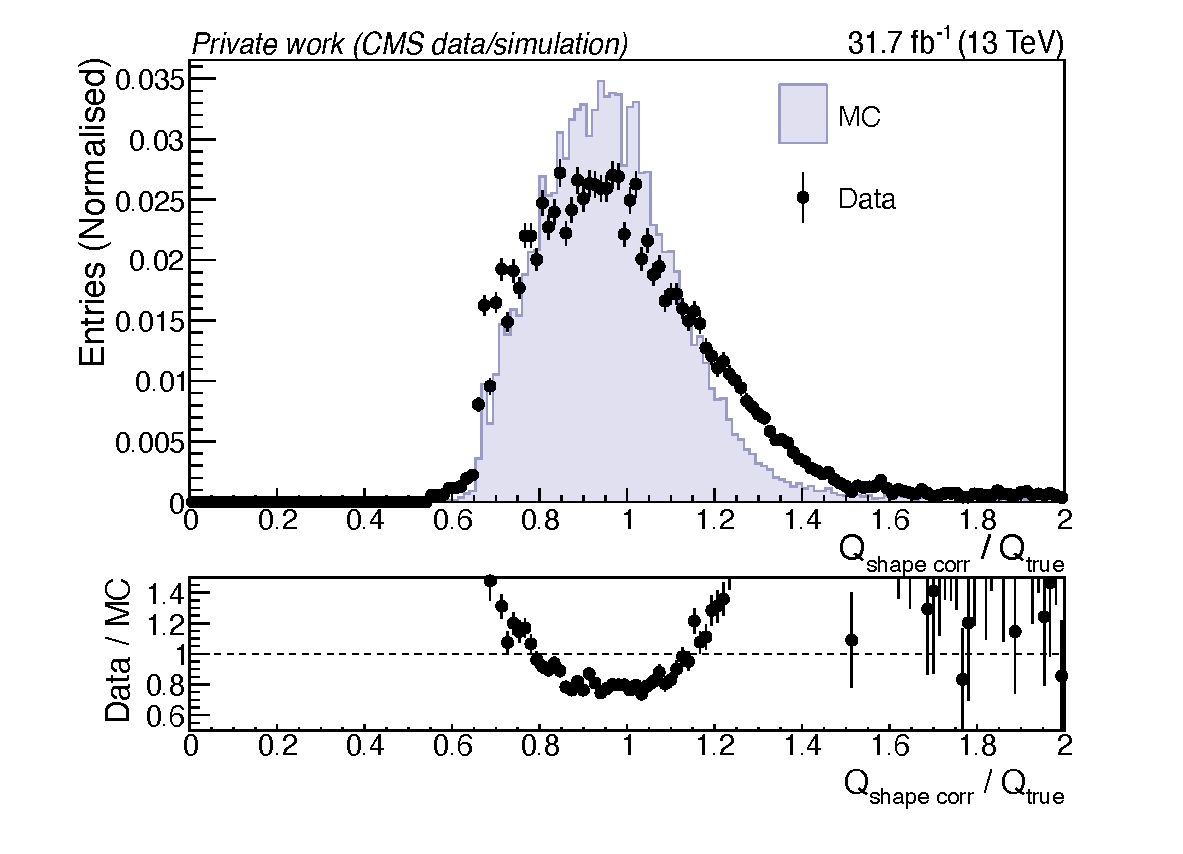
\includegraphics[width=0.49\linewidth,trim={0.8cm 0.5cm 1.5cm 0},clip]{Images/Ch2/NewCorr_dataVSmc_Wjets_weighted_bis.pdf}
    \caption{Rapport entre la charge corrigée $Q_\mathrm{corr}$ et la charge vraie $Q_\mathrm{true}$ pour des amas de données (points) et de la simulation $W$+jets (histogramme), dont le maximum vrai est compris entre 240 et 250 coups ADC, et artificiellement saturés à 240 coups ADC, avec la correction de base (à gauche) et la correction par forme (à droite). Les panneaux inférieurs montrent le rapport données/simulation.}
    \label{fig:resume:validation}
\end{figure}

Certaines limites de ma méthode demeurent. Les coefficients ont été calibrés et validés dans différents régimes de charge, sur un échantillon MC--muon de taille limitée. Par ailleurs, une partie des amas \textit{Left} et \textit{Right}, où la charge est fortement partagée entre le maximum et ses voisines, est surcorrigée, et la modification des critères de classification dégrade en contrepartie la correction des amas \textit{Center}. Une régression par un réseau de neurones peu profond, prenant en entrée la forme de l'amas, les charges voisines et la position de son barycentre, permettrait de se passer de cette classification.

\begin{table}[h!]
    \centering
    \small
    \renewcommand{\arraystretch}{1.3}
    \begin{tabular}{lcccc}
        \toprule
        & \multicolumn{2}{c}{Correction de base} & \multicolumn{2}{c}{Correction par forme} \\
        \cmidrule(lr){2-3} \cmidrule(lr){4-5}
        & Données & Simulation & Données & Simulation \\
        \midrule
        Moyenne de $Q_\mathrm{corr}/Q_\mathrm{true}$ & 0,92 & 0,88 & 0,99 & 0,97 \\
        Écart-type de $Q_\mathrm{corr}/Q_\mathrm{true}$ & 0,22 & 0,19 & 0,21 & 0,17 \\
        Amas restant sous 240 coups ADC & 12,5\,\% & 16,8\,\% & 1,7\,\% & 1,4\,\% \\
        Fraction d'amas corrigés & 73,1\,\% & 72,2\,\% & 94,4\,\% & 95,1\,\% \\
        \bottomrule
    \end{tabular}
    \caption{Comparaison des deux corrections de saturation sur les amas des données de 2018 et de la simulation $W$+jets, artificiellement saturés à 240 coups ADC.}
    \label{tab:resume:correction}
\end{table}


\subsection{Performances avec les données 2024--2025 et impact sur la recherche de HSCP}

La correction par forme, approuvée par les groupes de performance du trajectographe de CMS, a servi aux résultats publics de performance en \dedx{} obtenus à partir des données de 2024~\cite{CMS-DP-2025-020} et de 2025~\cite{CMS-DP-2026-102}. Dans ces études, la distribution de $I_h$ pour des traces \textit{HighPurity} à basse impulsion est ajustée, par intervalle de $p$, par une fonction de Landau convoluée avec une gaussienne ; la dépendance en $\beta\gamma$ est ensuite décrite par une paramétrisation empirique à cinq paramètres, ajustée sur la bande des protons et extrapolée aux autres espèces (\hyperref[fig:resume:dedxp]{Figure~\ref*{fig:resume:dedxp}}). La correction par forme donne des valeurs de \dedx{} plus élevées que la correction de base à basse impulsion, où la fraction d'amas saturés est la plus grande, et identiques au-delà.

\begin{figure}[h!]
    \centering
    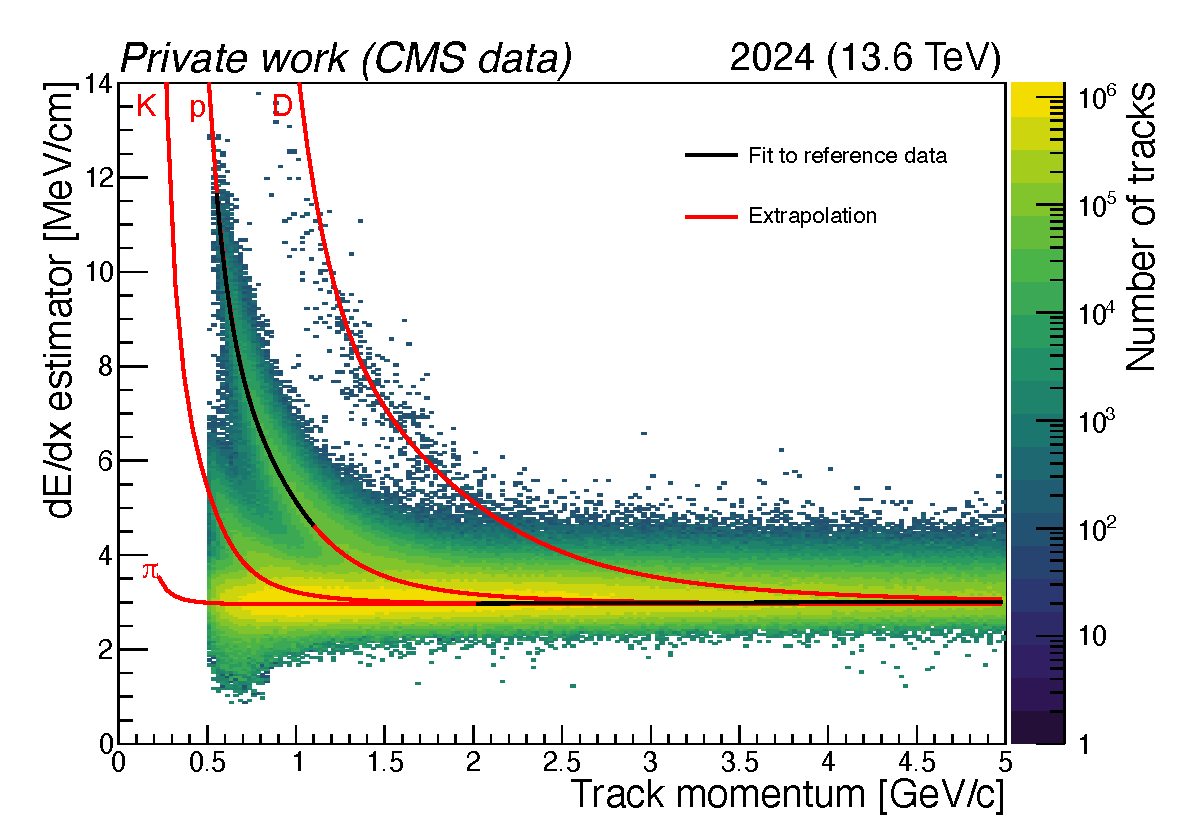
\includegraphics[width=0.49\linewidth]{Images/Ch2/dEdX0stripVsP_lowp_FIT_A_oldcorr.pdf}
    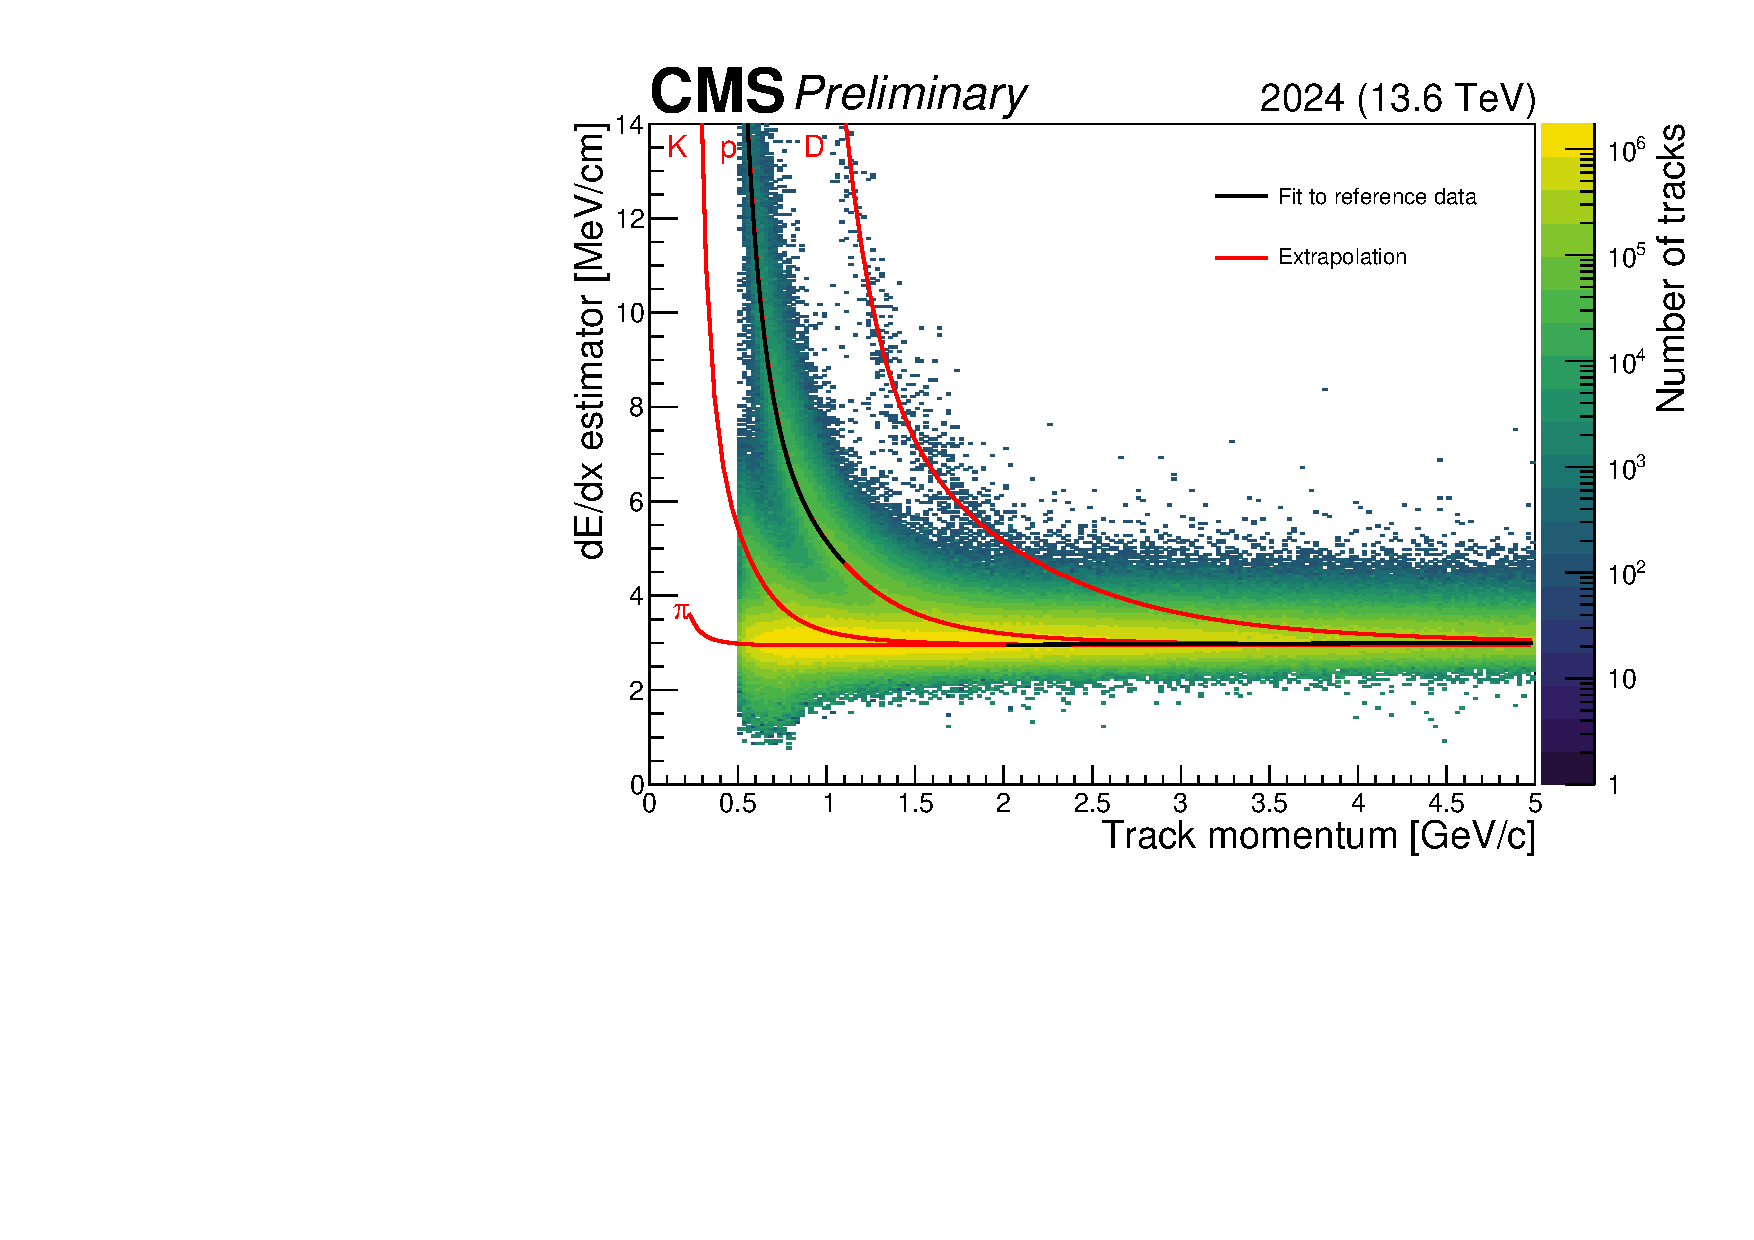
\includegraphics[width=0.49\linewidth]{Images/Ch2/dEdX0stripVsP_lowp_FIT_A.pdf}
    \caption{Estimateur $I_h$ en fonction de l'impulsion des traces dans les données de 2024, avec la correction de base (à gauche) et la correction par forme (à droite)~\cite{CMS-DP-2025-020}. Les courbes noires correspondent à l'ajustement sur la bande de référence, les courbes rouges à son extrapolation aux pions, aux kaons, aux protons et aux deutons.}
    \label{fig:resume:dedxp}
\end{figure}

L'impact sur la recherche de HSCP se mesure à partir de la masse reconstruite des gluinos simulés de 2000~GeV (\hyperref[fig:resume:massehscp]{Figure~\ref*{fig:resume:massehscp}}). La masse est obtenue en résolvant numériquement, par la méthode de Brent~\cite{brent2002}, l'équation $f(\beta\gamma)=I_h$, où $f$ est la paramétrisation empirique à cinq paramètres ajustée sur le signal. Sans correction, la masse moyenne reconstruite vaut 1688~GeV ; elle atteint 1900~GeV avec la correction de base et 2053~GeV avec la correction par forme, la plus proche de la masse générée. Une mesure non biaisée de l'ionisation permet donc de déterminer la masse. Dans l'analyse, la paramétrisation est calibrée sur des particules du MS, ce qui introduit un biais résiduel sans conséquence sur l'interprétation statistique (\hyperref[subsec:resume:masse]{Section~\ref*{subsec:resume:masse}}).

\begin{figure}[h!]
    \centering
    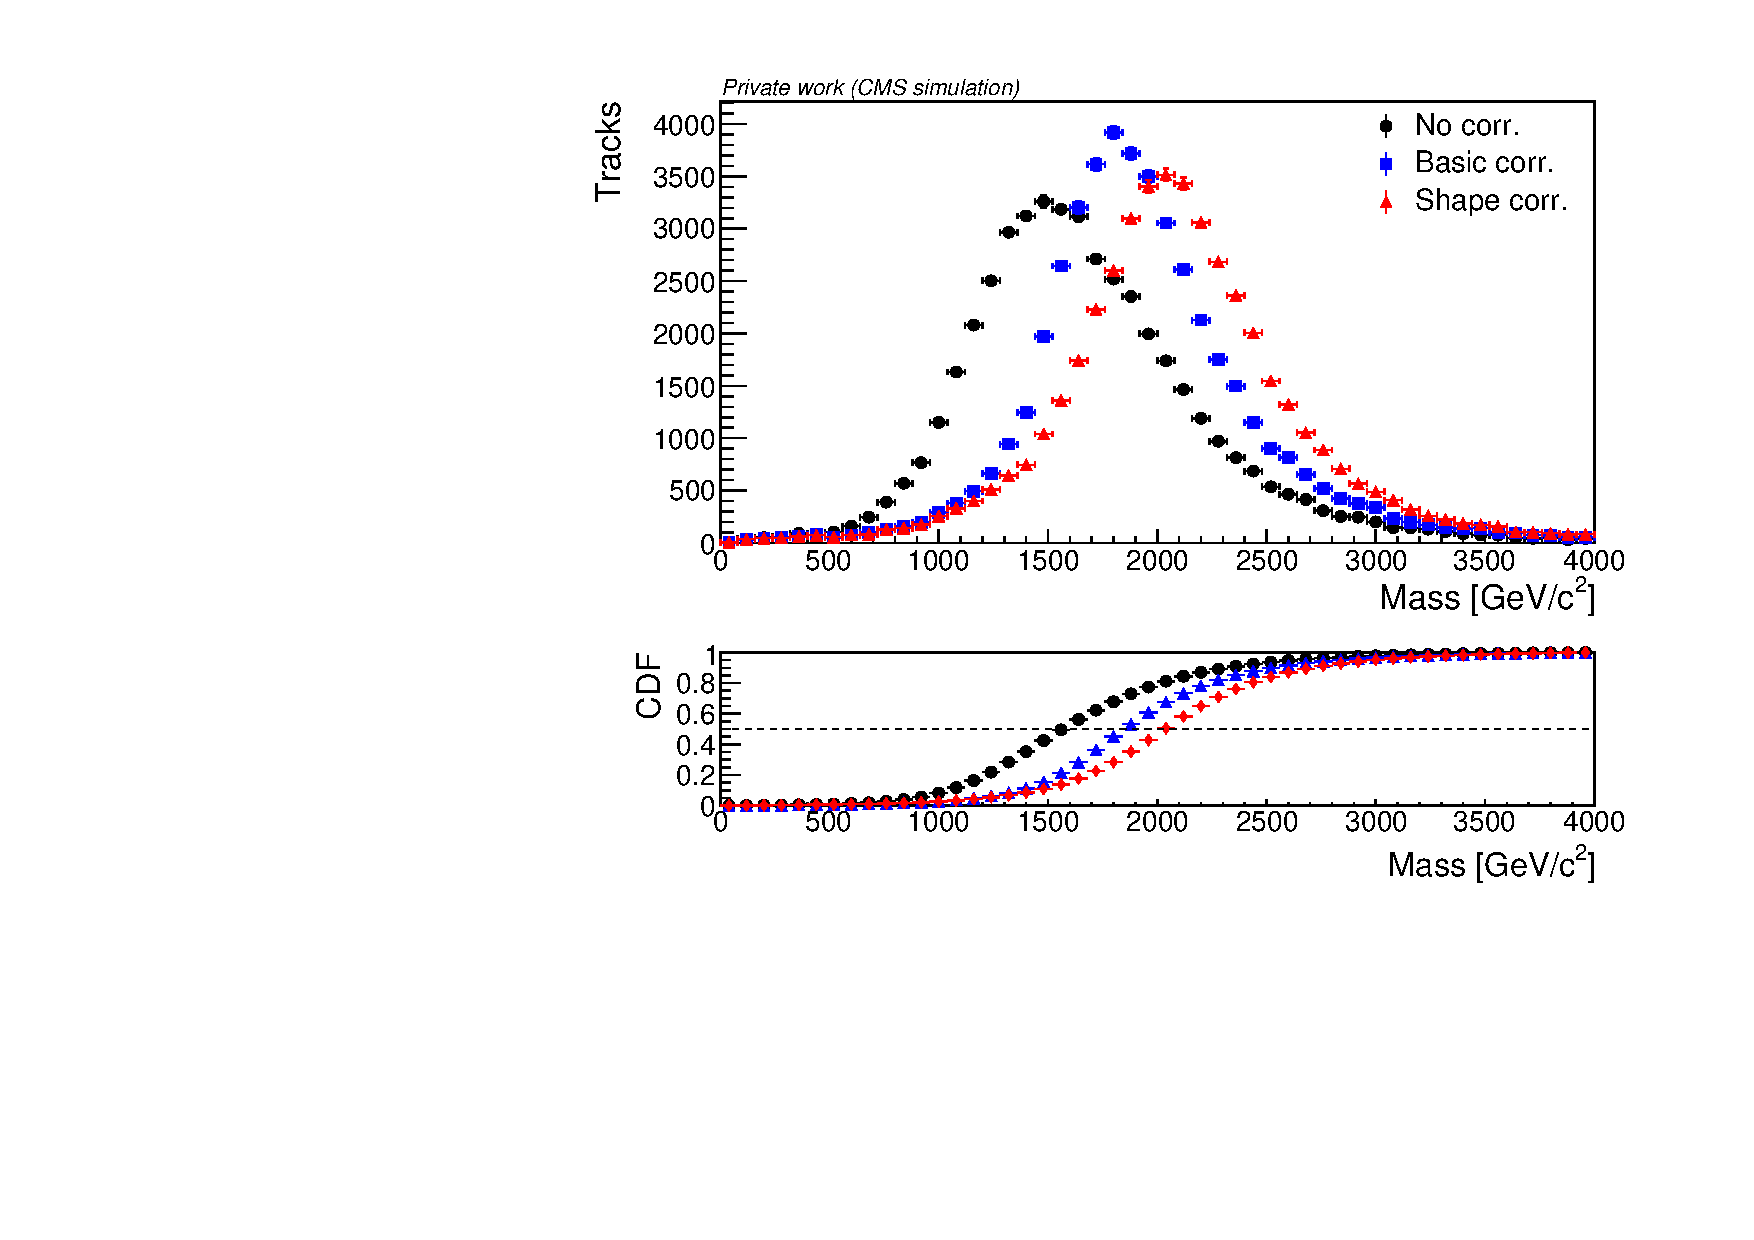
\includegraphics[width=0.75\linewidth]{Images/Ch2/Mass_HSCP_bis.pdf}
    \caption{Masse reconstruite des traces de gluinos simulés ($m_{\tilde{g}}=2000$~GeV) sans correction de saturation (cercles noirs), avec la correction de base (carrés bleus) et avec la correction par forme (triangles rouges). Le panneau inférieur présente les distributions cumulées.}
    \label{fig:resume:massehscp}
\end{figure}


%% ---------------------------------------------------------------------
\section{Cadre théorique et contexte expérimental}
\label{sec:resume:theorie}

\subsection{Le Modèle Standard et ses limites}

Le MS~\cite{Glashow1961, Weinberg1967, Salam1968} est une théorie quantique des champs fondée sur le groupe de jauge $\mathrm{SU}(3)_c\otimes\mathrm{SU}(2)_L\otimes\mathrm{U}(1)_Y$. Les fermions (quarks et leptons, répartis en trois générations) constituent la matière ; les bosons de jauge, imposés par l'invariance sous des transformations de jauge locales, véhiculent les interactions : le photon, les bosons $W^\pm$ et $Z^0$, et huit gluons porteurs d'une charge de couleur. L'interaction faible, qui viole la parité au maximum, n'agit que sur les fermions de chiralité gauche et s'unifie avec l'électromagnétisme dans le groupe $\mathrm{SU}(2)_L\otimes\mathrm{U}(1)_Y$. La brisure spontanée de cette symétrie par le mécanisme de Brout-Englert-Higgs donne leur masse aux bosons $W^\pm$ et $Z^0$ et prédit le boson de Higgs ; les fermions chargés acquièrent la leur par leurs couplages de Yukawa avec le doublet de Higgs. Le MS comporte 19 paramètres libres, déterminés expérimentalement.

Malgré l'accord de ses prédictions avec les mesures sur plus de quatorze ordres de grandeur en matière de section efficace, le MS n'explique ni la masse des neutrinos, mise en évidence par leurs oscillations, ni l'asymétrie baryonique de l'Univers, ni la matière noire (environ 27\,\% du contenu énergétique de l'Univers) ni l'énergie sombre (environ 68\,\%). La masse du boson de Higgs reçoit en outre des corrections radiatives proportionnelles au carré de l'échelle d'énergie la plus élevée de la théorie : la maintenir à 125~GeV face à l'échelle de Planck exige un ajustement fin d'une précision relative de $10^{-34}$ ; c'est le problème de la hiérarchie. Enfin, la gravitation n'est pas décrite.

\subsection{La supersymétrie}

La supersymétrie (SUSY)~\cite{ELLIS1984453,Ellis:591472} attribue à chaque particule du MS un partenaire dont le spin diffère d'une demi-unité, tels que les squarks et sleptons scalaires, ainsi que les jauginos (y compris le gluino) et les higgsinos fermioniques. Dans l'extension supersymétrique minimale du MS (MSSM), qui requiert deux doublets de Higgs, les partenaires des bosons électrofaibles et des bosons de Higgs se mélangent en charginos et en neutralinos. Si la $R$-parité est conservée, la particule supersymétrique la plus légère est stable ; s'il s'agit du neutralino le plus léger, il est un candidat naturel pour la matière noire. Les contributions des bosons et des fermions aux corrections de la masse du Higgs se compensant, le problème de la hiérarchie est résolu si les superpartenaires ont des masses de l'ordre du TeV, accessibles au LHC. La brisure «~douce~» de la SUSY introduit toutefois 105 paramètres libres, ce qui conduit les expériences à interpréter leurs résultats dans des modèles simplifiés.

\subsection{Particules à long temps de vie}

Les temps de vie des particules du MS s'étendent sur plus de cinquante ordres de grandeur. Une particule dont la longueur de vie propre $c\tau$ est bien inférieure à la résolution du trajectographe est dite prompte ; au-delà de la taille du système à muons (environ 10~m), elle est stable à l'échelle du détecteur. Trois mécanismes peuvent induire une longue durée de vie de nouvelles particules : un couplage très faible (par exemple, un neutralino se désintégrant via un couplage $\lambda$ qui viole la $R$-parité, avec $\tau\propto1/\lambda^2$), un médiateur très lourd, ou un spectre comprimé qui réduit l'espace des phases. Dans le scénario de \textit{split} SUSY~\cite{ArkaniHamed:2004fb, Giudice:2004tc}, où les scalaires ont une masse $m_S\gg1$~TeV, le gluino ne peut se désintégrer que par l'intermédiaire de squarks virtuels, avec
\begin{equation}
    \tau_{\tilde{g}} \, [\mathrm{s}] \,\approx 8\times\left(\frac{m_S}{10^9~\mathrm{GeV}}\right)^4\left(\frac{1~\mathrm{TeV}}{m_{\tilde{g}}}\right)^5 \, ,
\end{equation}
ce qui le rend stable à l'échelle du détecteur sur une large partie de l'espace des paramètres.

Les recherches de LLP de CMS sont organisées par signature : objets ou vertex déplacés, traces qui disparaissent, signaux retardés, gerbes dans le système à muons, … Pour des temps de vie supérieurs à la taille du détecteur, la signature de particules chargées devient une trace isolée de grande impulsion traversant tout l'appareillage : c'est celle étudiée dans cette thèse.

\subsection{Les particules lourdes, stables et chargées}

Les HSCP se répartissent en deux familles~\cite{Fairbairn:2006gg}. Les HSCP de type hadronique, comme le gluino ou le stop (partenaire du quark top) à long temps de vie, portent une charge de couleur et s'hadronisent en $R$-hadrons : $R$-mésons, $R$-baryons et, pour le gluino, des états gluino-gluon neutres (\textit{gluinoballs}). Au cours de leur propagation, les interactions nucléaires avec la matière du détecteur peuvent modifier leur composition en quarks, et donc leur charge électrique : un $R$-hadron chargé peut devenir neutre, et inversement (\textit{charge flipping})~\cite{Mackeprang:2009ad}. Les HSCP de type leptonique, comme le stau des modèles à brisure de supersymétrie par médiation de jauge (GMSB) ou des leptons de quatrième génération $\tau'$ de charge $e$ ou $2e$, ne sont soumis qu'à l'interaction électrofaible et se comportent comme des muons lourds. À masse égale, la section efficace de production de paires de gluinos, favorisée par la structure en octet de couleur, est nettement plus grande que celle des stops, et bien supérieure à celle des HSCP de type leptonique (\hyperref[fig:resume:xsec]{Figure~\ref*{fig:resume:xsec}}).

\begin{figure}[htbp]
    \centering
    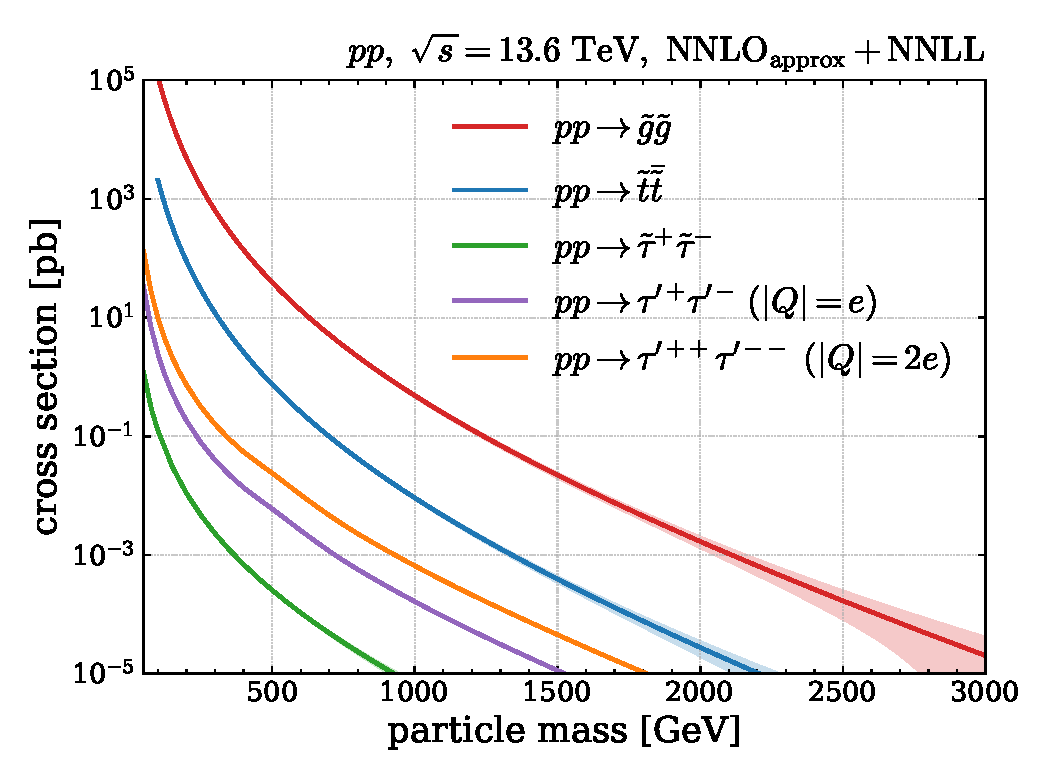
\includegraphics[width=0.8\linewidth]{Images/Ch3/xsec_theory.pdf}
    \caption{Sections efficaces théoriques de production de paires (NNLO$_\mathrm{approx}$+NNLL) à $\sqrt{s}=13{,}6$~TeV pour les gluinos, les stops, les staus et les leptons $\tau'$ de charge $e$ ou $2e$, en fonction de leur masse~\cite{10.21468/SciPostPhysCore.7.4.072, Fiaschi_2023}. Les bandes indiquent l'incertitude théorique.}
    \label{fig:resume:xsec}
\end{figure}

Leur masse élevée rend les HSCP lentes, avec typiquement $0{,}1\lesssim\beta\gamma\lesssim1$. Trois observables en découlent : une ionisation anormalement élevée dans le trajectographe, observable principale de cette thèse ; un temps de vol allongé jusqu'au système à muons ; et, pour les $R$-hadrons, de la MET lorsque la paire produite comprend un $R$-hadron chargé et un $R$-hadron neutre, ce dernier échappant à la détection. Trop lents, les $R$-hadrons chargés atteignent souvent le système à muons en dehors de la fenêtre de temps de déclenchement des muons.

\subsection{État des recherches de HSCP}

La dernière recherche de la collaboration CMS, menée avec 101~fb$^{-1}$ de données du Run--2 enregistrées en 2017 et 2018~\cite{HSCP_Run2}, combinait deux méthodes : l'une fondée sur la masse reconstruite à partir de l'impulsion et de l'ionisation dans les pistes, l'autre fondée sur l'ionisation seule, exploitant l'indépendance des mesures des pixels et des pistes. Les événements y étaient sélectionnés par des déclencheurs sur les muons, et la recherche était restreinte au tonneau ($|\eta|<1$). Aucun excès n'ayant été observé, les gluinos stables ont été exclus jusqu'à 2,08~TeV, les stops jusqu'à 1,47~TeV et les staus GMSB jusqu'à 0,85~TeV (limites observées par la méthode de masse). Du côté d'ATLAS, l'analyse de 139~fb$^{-1}$ du Run--2~\cite{HSCP_ATLAS_2022} a relevé sept événements dans une fenêtre de masse de 1,1 à 2,8~TeV pour $0{,}7\pm0{,}4$ attendus, soit un excès de $3{,}6\sigma$ localement ($3{,}3\sigma$ globalement) ; la vitesse mesurée des candidats ($\beta\gamma\approx1$) est toutefois peu compatible avec des $R$-hadrons lents. La recherche de CMS a testé l'interprétation alternative en termes de leptons $\tau'$ de charge $2e$ issus de la désintégration d'un boson $Z'$ lourd~\cite{Giudice:2022bpq}, sans la confirmer. Une analyse plus récente d'ATLAS~\cite{HSCP_ATLAS_2025}, qui combine l'ionisation dans les pixels et le temps de vol dans le calorimètre, exclut les gluinos stables jusqu'à environ 2,20~TeV.


%% ---------------------------------------------------------------------
\section{Recherche de HSCP avec les données du Run--3}
\label{sec:resume:analyse}

\subsection{Stratégie et échantillons}

La recherche présentée dans cette thèse porte sur les $R$-hadrons issus de la production de paires de gluinos. Elle lève les deux principales limitations de l'analyse du Run--2 de la collaboration CMS grâce à une sélection d'événements fondée sur des déclencheurs MET plutôt que sur les muons, et à une acceptance étendue à toute la couverture du trajectographe ($|\eta|<2{,}4$). Au-delà de ces changements, la présélection suit celle du Run--2. Les échantillons de signal ont été produits par d'autres membres de l'équipe. Pour ma part, j'ai défini la stratégie de déclenchement, développé la méthode d'estimation du bruit de fond, évalué les incertitudes systématiques et calculé les limites d'exclusion.

Les données analysées ont été enregistrées en 2024 (ères C à I) à $\sqrt{s}=13{,}6$~TeV et correspondent à 109~fb$^{-1}$. Le signal est simulé pour dix hypothèses de masse de gluino comprises entre 1100 et 2600~GeV, avec une durée de vie infinie et une fraction de \textit{gluinoballs} de 10\,\% ; les sections efficaces sont calculées à l'ordre NNLO$_\mathrm{approx}$+NNLL~\cite{10.21468/SciPostPhysCore.7.4.072}. Les principaux bruits de fond simulés, $W(\to\mu\nu)$+jets, $t\bar{t}$ semi- et dileptonique, et la production multijet QCD enrichie en muons, servent uniquement à guider la présélection : le bruit de fond final est estimé à partir des données.

\subsection{Les discriminants d'ionisation \texorpdfstring{$F_\mathrm{pixel}$}{Fpixel} et \texorpdfstring{$I_h$}{Ih}}

L'analyse exploite séparément les mesures d'ionisation des pixels et des pistes. Dans le détecteur à pixels, le discriminant $F_\mathrm{pixel}$ quantifie la compatibilité d'une trace avec l'hypothèse MIP. Pour chaque amas de pixels de charge $Q$, on calcule la probabilité $p_Q$ qu'une MIP dépose une charge supérieure, à partir de gabarits de Vavilov issus de la simulation \texttt{PixelAV}~\cite{1495807} ; si le modèle est correct, $p_Q$ est uniformément distribuée sur l'intervalle [0, 1]. Le produit $\displaystyle \alpha_n=\prod_i p_{Q_i}$ sur les $n$ couches traversées n'est pas uniforme, mais $-\ln\alpha_n$ suit une loi Gamma de paramètres $(n,1)$, dont la fonction de répartition est connue analytiquement :
\begin{equation}
    \beta_n=\alpha_n\sum_{m=0}^{n-1}\frac{\left[-\ln\alpha_n\right]^m}{m!} ,
    \qquad
    F_\mathrm{pixel}=1-\beta_n .
\end{equation}
La variable $F_\mathrm{pixel}$ est ainsi uniforme pour les MIP quel que soit le nombre de couches, et tend vers 1 pour une particule fortement ionisante. La première couche du tonneau, trop dégradée par les rayonnements, est exclue du calcul.

Dans les pistes, l'ionisation est mesurée par l'estimateur $I_h$ de l'\hyperref[eq:resume:ih]{\'Equation~\ref*{eq:resume:ih}}. Il est calculé à partir de dépôts préalablement traités par la correction de saturation par forme que j'ai développée. Suivies tout au long de l'année 2024, les deux variables restent stables après l'étalonnage de la charge, à une légère dérive de $F_\mathrm{pixel}$ près, due au vieillissement des capteurs à pixels. Pour les traces du MS de grande impulsion, toutes relativistes, $F_\mathrm{pixel}$ et $I_h$ échantillonnent indépendamment les fluctuations des dépôts au niveau de la MIP et sont donc décorrélés ; pour les HSCP, les deux variables répondent au même excès d'ionisation. Cette propriété est utilisée pour estimer le bruit de fond.

\subsection{Stratégie de déclenchement}

Les gluinos simulés sont produits à une vitesse typique de $\beta\approx0{,}55$. Le déclenchement sur muon \texttt{HLT\_Mu50}, utilisé au Run--2, a un seuil d'efficacité situé vers $\beta\approx0{,}6$ (\hyperref[fig:resume:beta]{Figure~\ref*{fig:resume:beta}}) et ne retient qu'environ 11\,\% des événements de signal. La composition des paires aggrave cette perte : au niveau généré, 30\,\% des paires sont neutre-neutre, 50\,\% neutre-chargé et 20\,\% chargé-chargé, mais après association aux traces reconstruites, 40\,\% des événements n'ont aucune trace associée, 46\,\% une seule et 14\,\% deux. Ce déplacement traduit le passage de $R$-hadrons chargés à l'état neutre dans le détecteur. Dans 99\,\% des cas, la trace d'un $R$-hadron chargé est identifiée comme un muon PF.

\begin{figure}[h!]
    \centering
    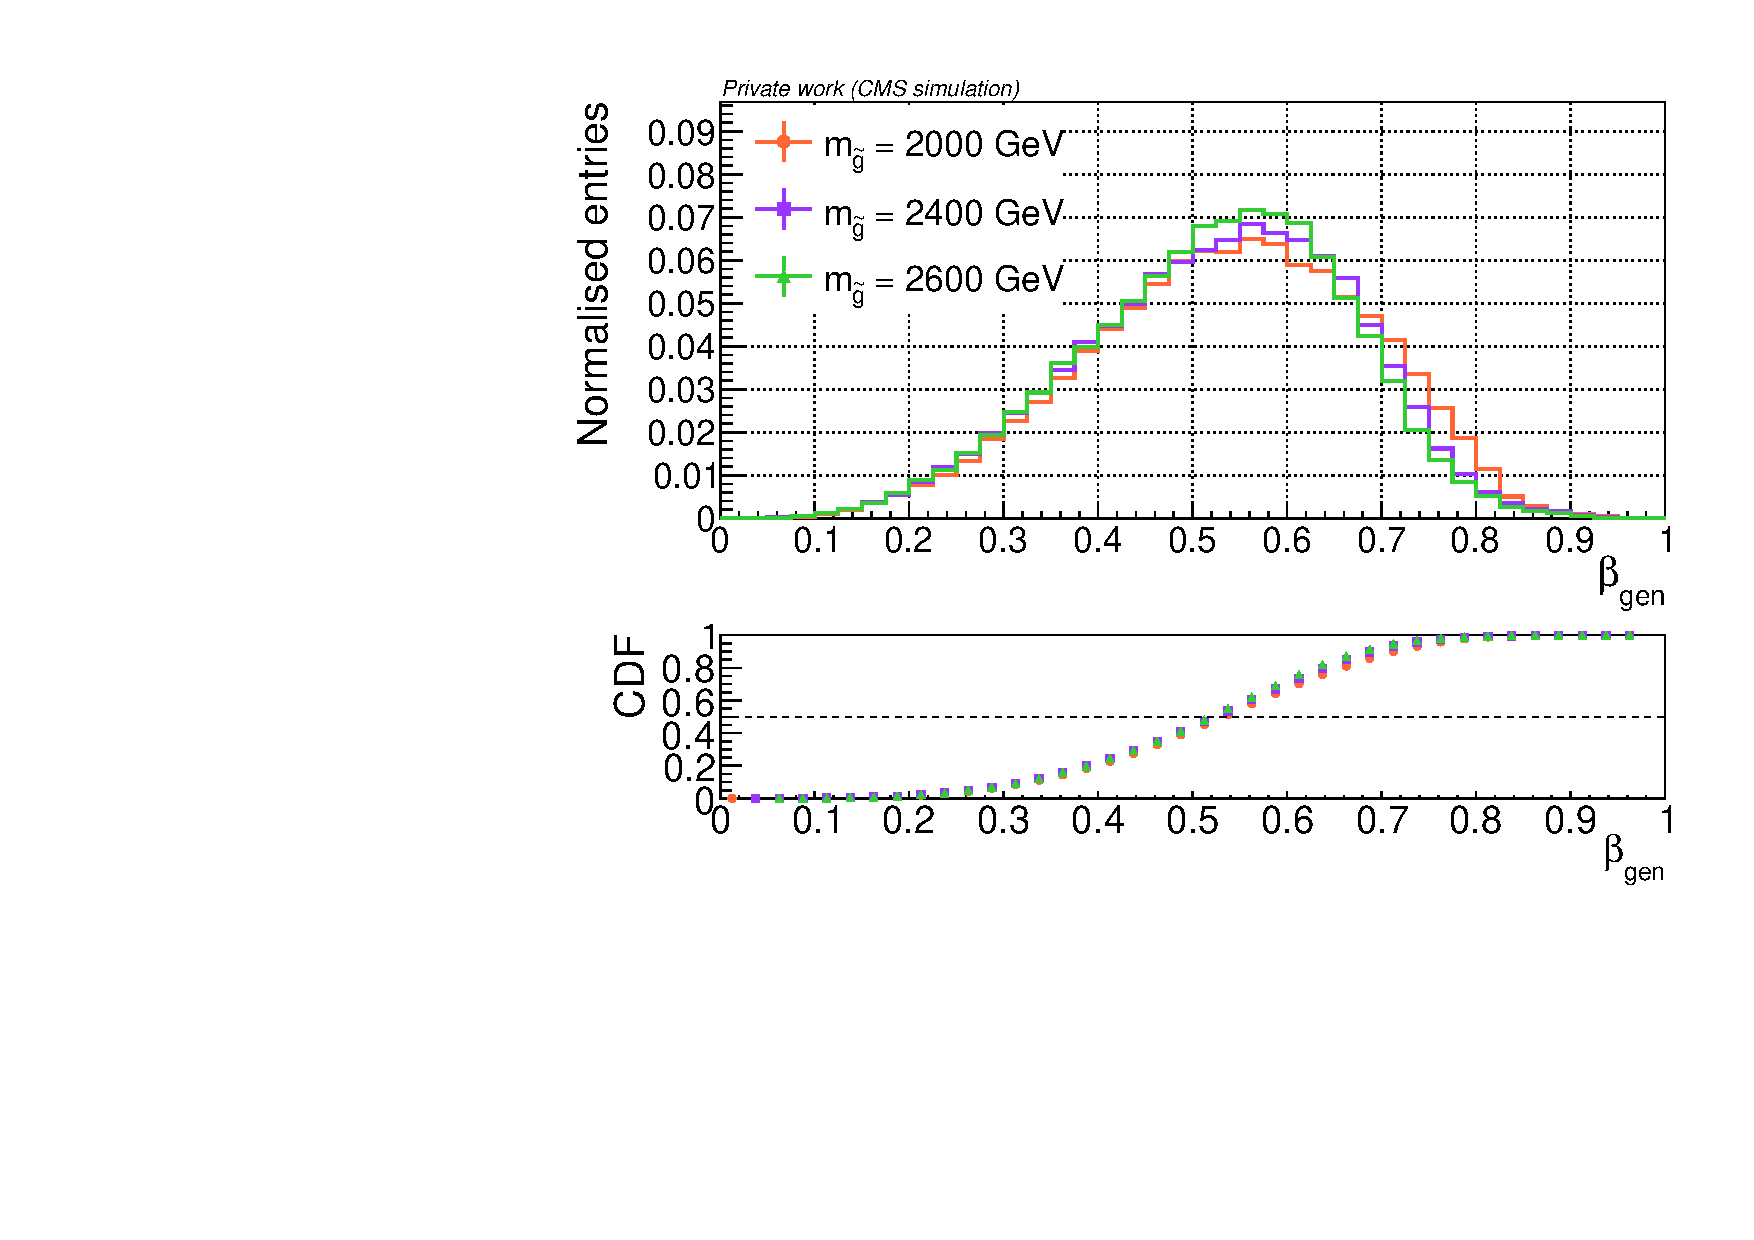
\includegraphics[width=0.49\linewidth,valign=c]{Images/Ch4/c_BetaDistribution__TriggEffBeta_bis.pdf}
    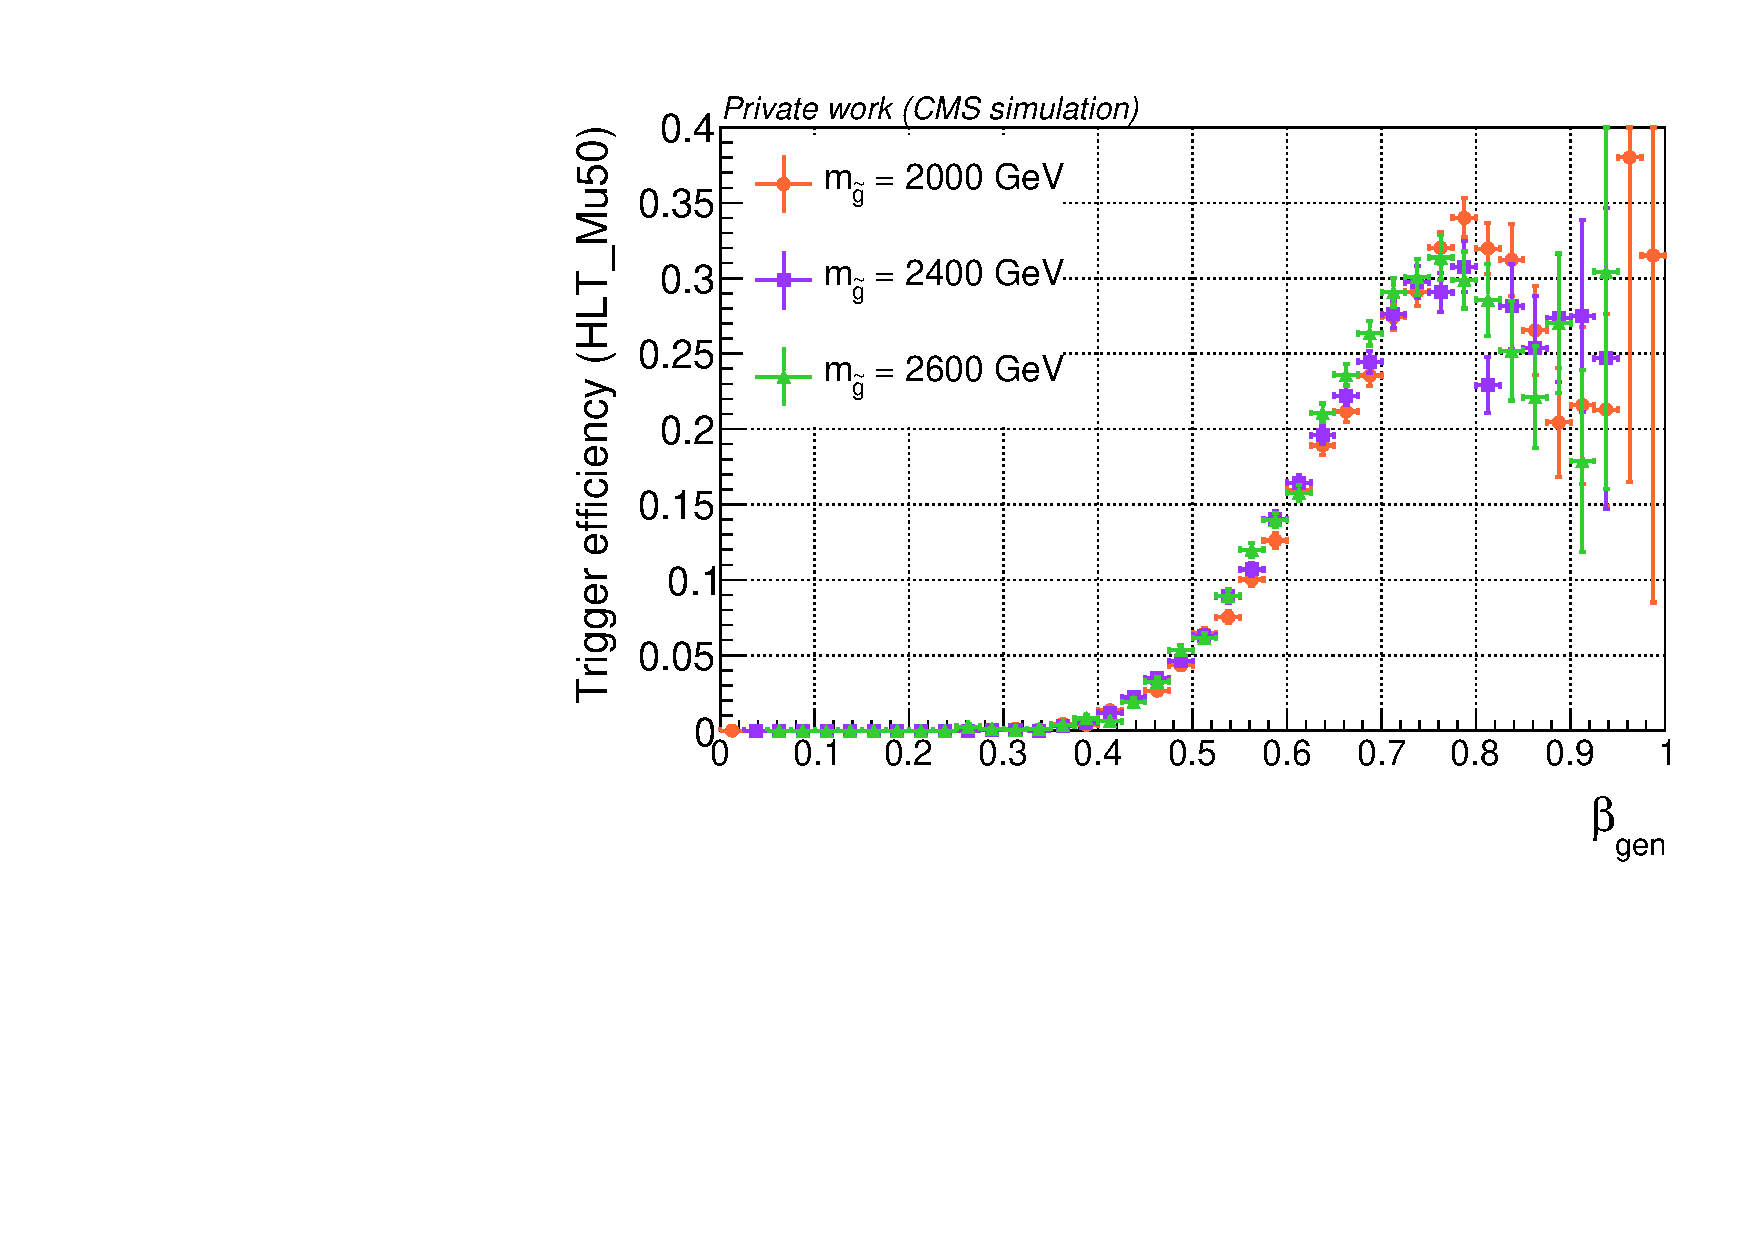
\includegraphics[width=0.49\linewidth,valign=c]{Images/Ch4/c_TriggerEfficiencyBeta__TriggEffBeta_bis.pdf}
    \caption{Distribution de la vitesse générée $\beta$ des gluinos pour trois hypothèses de masse (à gauche) et efficacité du déclenchement sur muon \texttt{HLT\_Mu50} en fonction de $\beta$ (à droite).}
    \label{fig:resume:beta}
\end{figure}

Une paire formée d'un $R$-hadron chargé et d'un $R$-hadron neutre produit un déséquilibre d'impulsion transverse, ce qui se traduit par une MET PF. De plus, les HSCP déposant très peu d'énergie dans les calorimètres, un jet issu d'un rayonnement dans l'état initial, qui recule contre la paire, engendre de la Calo MET. J'ai donc défini une stratégie fondée sur le «~ou~» logique de quatre chemins HLT portant sur les variables MET, MHT et $H_\mathrm{T}$, et la présence d'une trace isolée :
\begin{center}
    \small
    \texttt{HLT\_PFMET120\_PFMHT120\_IDTight}, \quad \texttt{HLT\_PFMETNoMu120\_PFMHTNoMu120\_IDTight\_PFHT60}, \\
    \texttt{HLT\_PFHT500\_PFMET100\_PFMHT100\_IDTight}, \quad \texttt{HLT\_MET105\_IsoTrk50}.
\end{center}
Leur combinaison sélectionne environ 30\,\% des événements de signal, soit près de trois fois plus que le déclenchement sur le muon, pour toutes les masses de gluino (\hyperref[fig:resume:trigger]{Figure~\ref*{fig:resume:trigger}}).

\begin{figure}[h!]
    \centering
    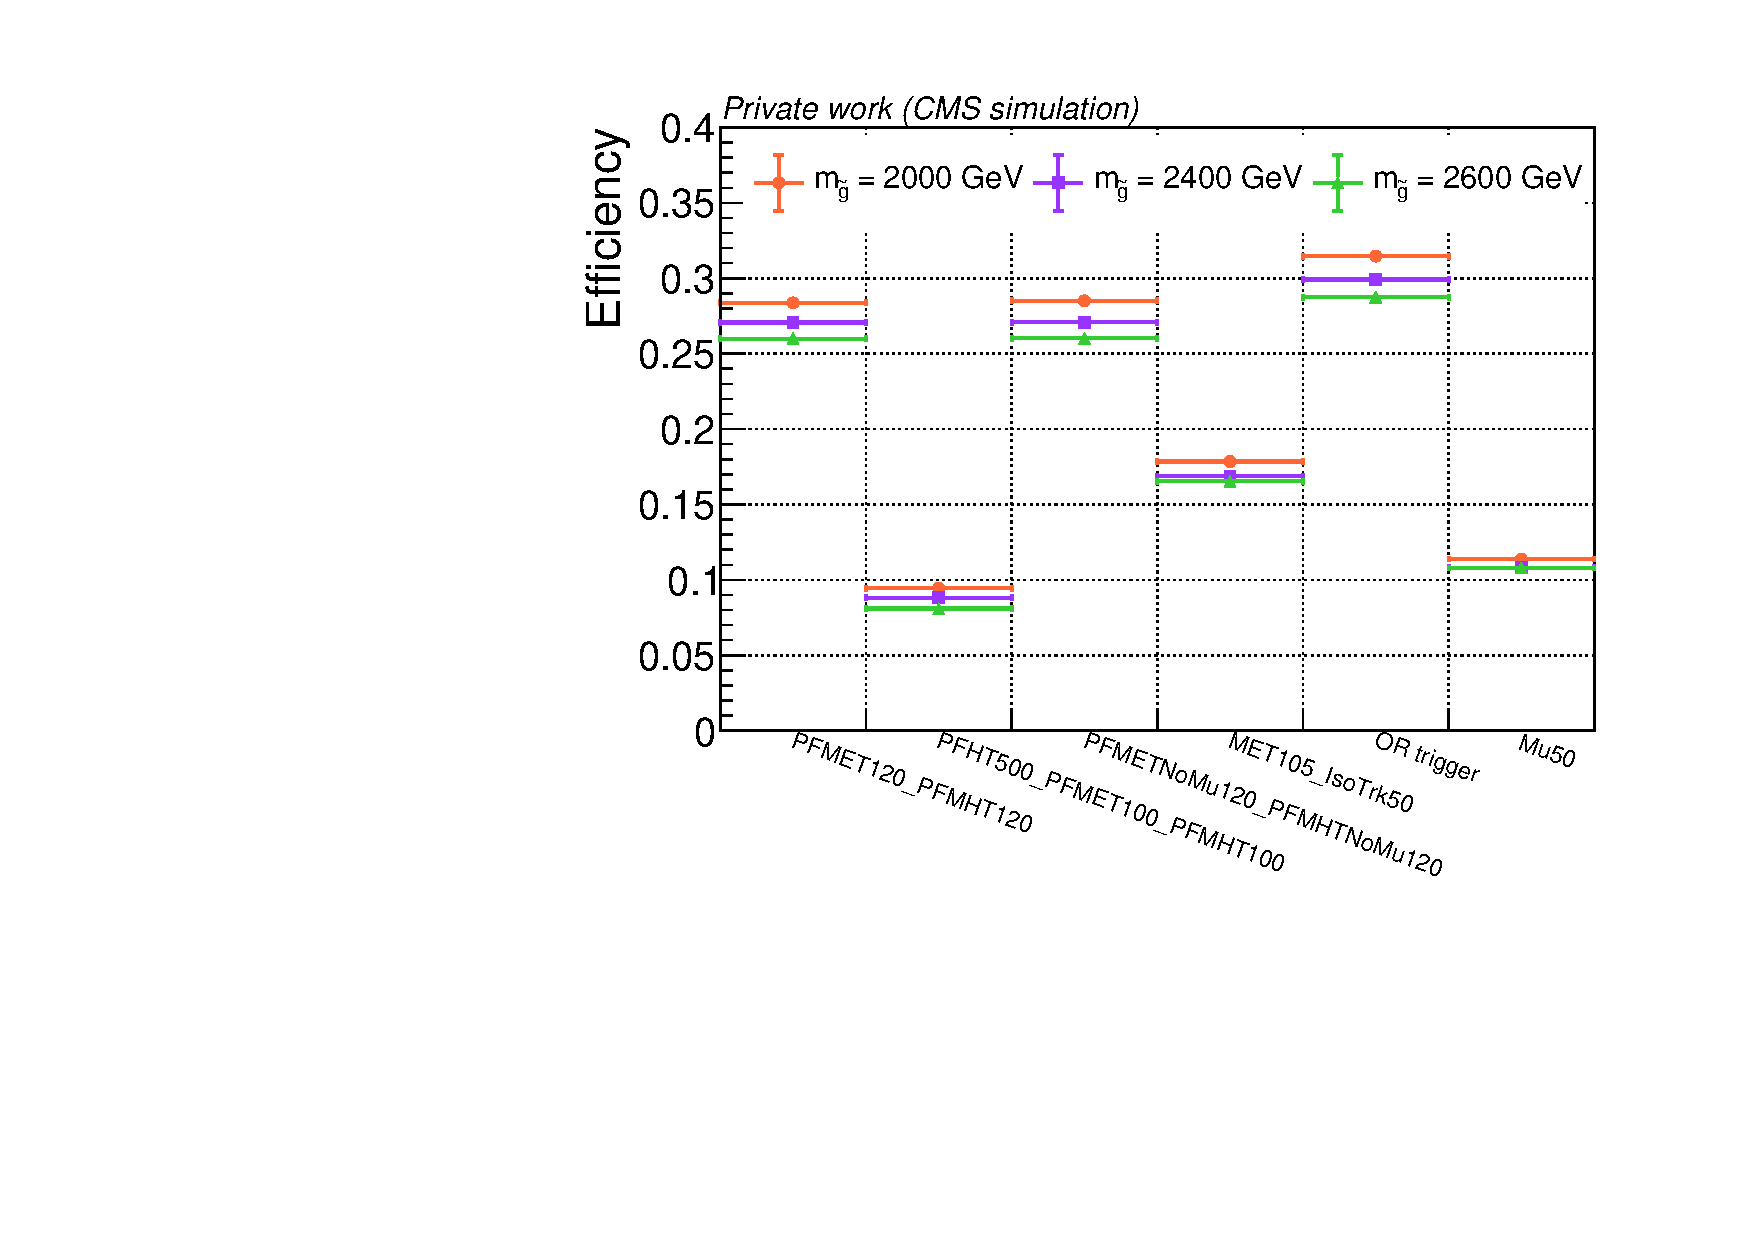
\includegraphics[width=0.49\linewidth,trim={0.8cm 0 1.2cm 0},clip]{Images/Ch4/c_TriggerEfficiency__TriggerEff_bis.pdf}
    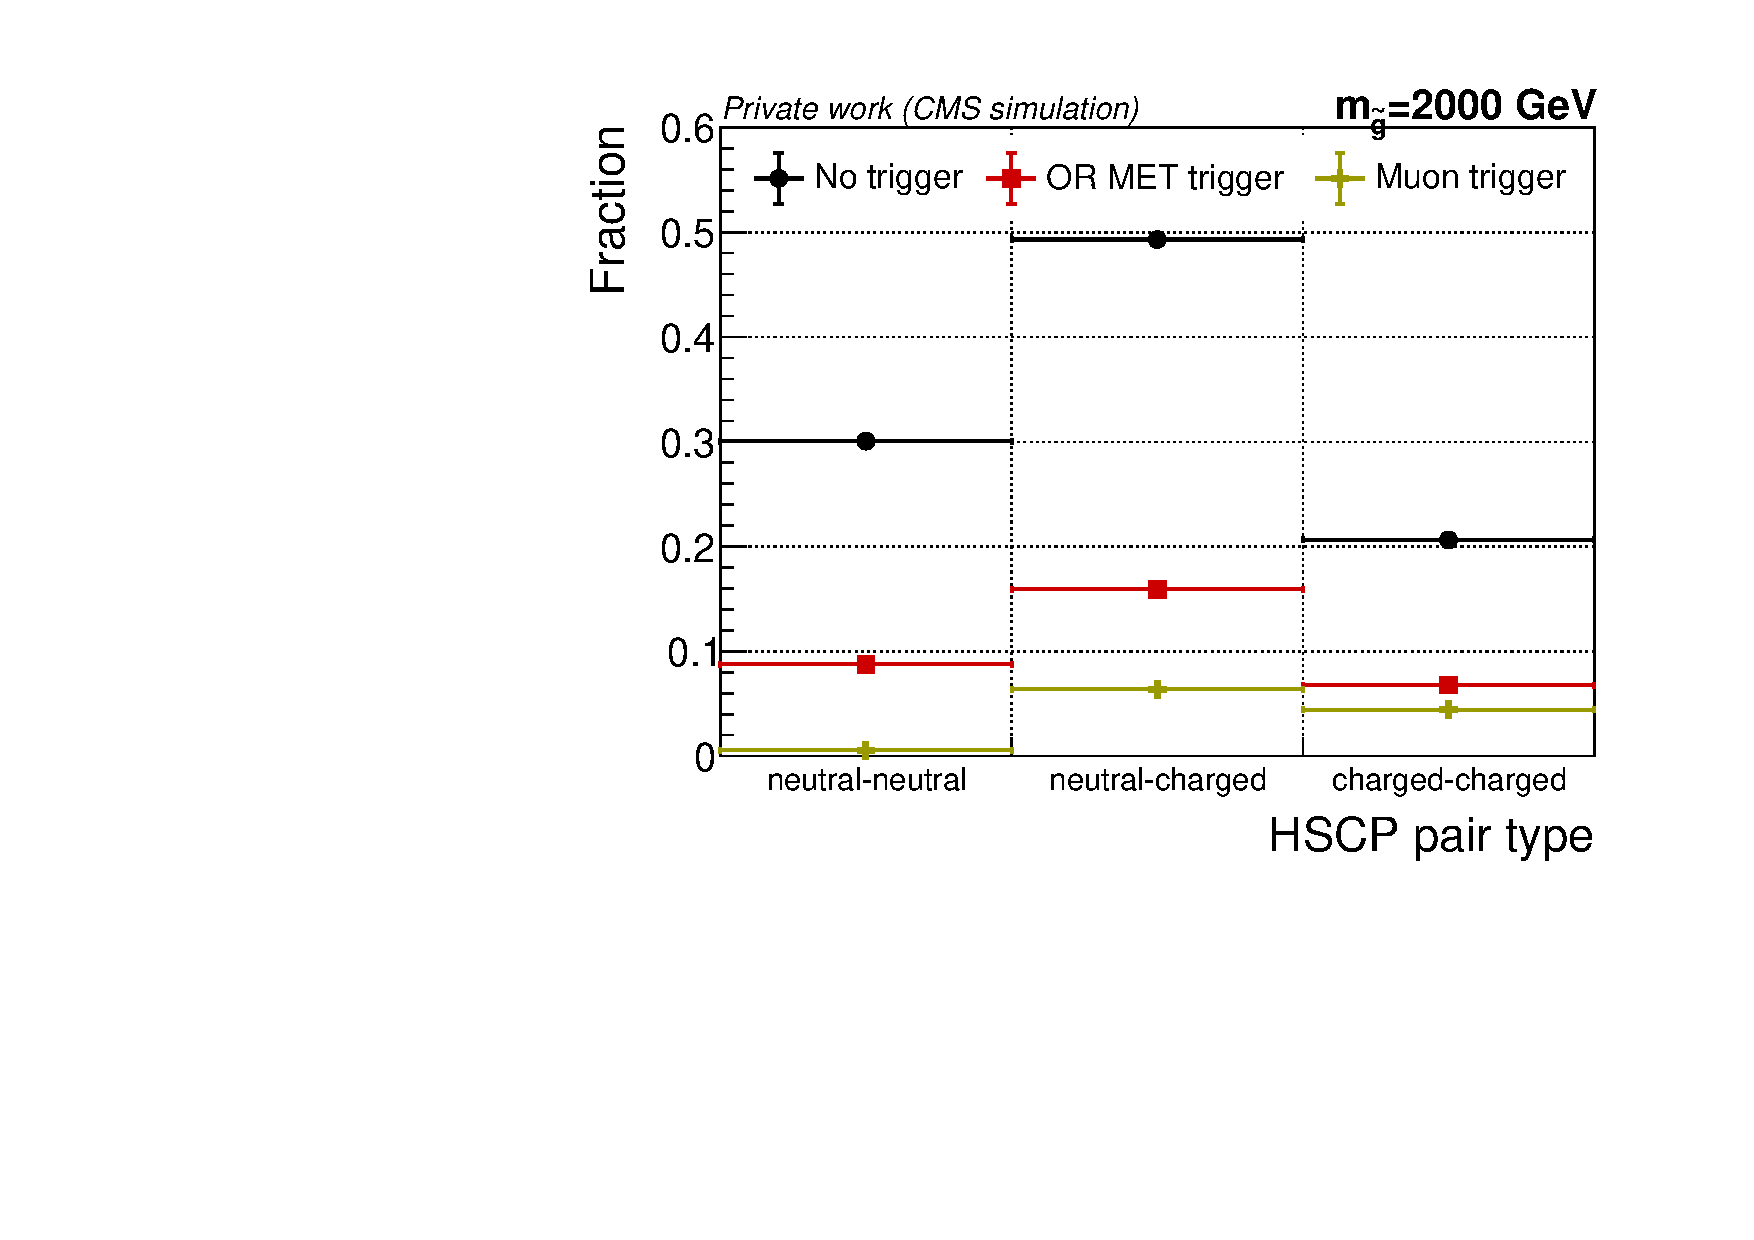
\includegraphics[width=0.49\linewidth,trim={0.8cm 0 1.2cm 0},clip]{Images/Ch4/PairTypeStages_SingleMass__Trigger_2000__PairTypeStages_bis.pdf}
    \caption{À gauche : efficacité des quatre chemins HLT fondés sur la MET, sur leur «~ou~» logique et du chemin \texttt{HLT\_Mu50}, pour plusieurs masses de gluino. À droite : composition des paires de HSCP ($m_{\tilde{g}}=2000$~GeV) au niveau généré (points noirs), soit après les déclenchements sur la MET (carrés rouges), soit après \texttt{HLT\_Mu50} (croix).}
    \label{fig:resume:trigger}
\end{figure}

L'efficacité de déclenchement dépend de quantités calculées «~en ligne~», alors que l'analyse utilise leurs équivalents «~hors ligne~». Dans la zone de montée de l'efficacité, un léger désaccord entre les données et la simulation rend la prédiction du nombre d'événements de signal peu fiable : il faut travailler sur le plateau, où le rapport des efficacités entre les données et la simulation (facteur d'échelle, SF) est constant. Dans le format de données utilisé pour l'analyse afin d'accéder aux dépôts \dedx des candidats HSCP, la Calo MET sauvegardée «~hors ligne~» inclut les dépôts des muons ; j'ai donc construit une variable approchée, la Pseudo MET, à partir de la somme vectorielle des jets calorimétriques afin de me rapprocher de la variable «~en ligne~». Les efficacités et les SF, mesurés dans un échantillon orthogonal de données sélectionnées par un déclenchement sur un muon isolé et dans une simulation $W\to\mu\nu$, deviennent constants au-delà de 250~GeV de Pseudo MET ou de 150~GeV de MET PUppi. Cette coupure sur la Pseudo MET non étalonnée ne conserverait qu'environ 40\,\% du signal déclenché, contre 85\,\% pour une coupure sur la MET PUppi. La stratégie retenue impose donc une MET PUppi supérieure à 150~GeV et corrige la simulation par des SF en fonction de cette variable, dont les incertitudes statistiques définissent l'incertitude systématique associée.

\subsection{Présélection}

La présélection, héritée de l'analyse des données du Run--2, à l'exception du déclenchement et de l'acceptance en $\eta$, requiert au moins une trace de $p_\mathrm{T}>50$~GeV et $|\eta|<2{,}4$, comptant au moins deux impacts dans les pixels, au moins dix mesures de \dedx, plus de 80\,\% d'impacts valides, la qualité \textit{HighPurity} et $\chi^2/N_\mathrm{dof}<5$. La trace doit être compatible avec le vertex primaire ($|d_z|<0{,}1$~cm, $|d_{xy}|<0{,}02$~cm) et isolée ($I_\mathrm{rel}^\mathrm{PF}<0{,}02$, $I_\mathrm{trk}<15$~GeV). La condition $E/p<0{,}3$ rejette les électrons, deux critères de résolution en impulsion éliminent les traces mal mesurées, et $F_\mathrm{pixel}>0{,}3$ écarte les amas de pixels scindés. Enfin, $I_h$ doit dépasser le seuil $C_\mathrm{mass}$ défini ci-dessous ; si plusieurs candidats subsistent, celui présentant la plus grande ionisation est retenu.

Le \hyperref[tab:resume:cutflow]{Tableau~\ref*{tab:resume:cutflow}} résume l'effet des principales coupures. La présélection réduit le nombre d'événements des données de près de quatre ordres de grandeur tout en conservant 11,6\,\% du signal pour $m_{\tilde{g}}=2000$~GeV, contre 4,8\,\% dans l'analyse du Run--2. Ce gain d'un facteur supérieur à deux provient du déclenchement sur la MET et de l'extension en $\eta$, qui porte l'acceptance d'environ 8,5\,\% pour le tonneau seul à 11,6\,\%.

\begin{table}[h!]
    \centering
    \small
    \renewcommand{\arraystretch}{1.25}
    \begin{tabular}{lcc}
        \toprule
        Critère (cumulé) & Données MET 2024 (\%) & $m_{\tilde{g}}=2000$~GeV (\%) \\
        \midrule
        Déclenchement MET («~ou~» logique) & 9,64 & 31,5 \\
        Filtres MET, MET PUppi $>150$~GeV & 4,29 & 25,8 \\
        $p_\mathrm{T}>50$~GeV, $|\eta|<2{,}4$ & 0,53 & 18,5 \\
        Qualité de la trace et vertex primaire & 0,39 & 16,0 \\
        Isolation ($I_\mathrm{rel}^\mathrm{PF}$, $I_\mathrm{trk}$) & 0,042 & 12,0 \\
        $E/p$ et résolution en impulsion & 0,022 & 11,7 \\
        $F_\mathrm{pixel}>0{,}3$ et $I_h>C_\mathrm{mass}$ & 0,018 & 11,6 \\
        \bottomrule
    \end{tabular}
    \caption{Efficacités cumulées des principaux critères de présélection pour les données de 2024 et pour des gluinos de 2000~GeV.}
    \label{tab:resume:cutflow}
\end{table}

\subsection{Reconstruction de la masse}
\label{subsec:resume:masse}

Dans le domaine d'impulsion des candidats, la perte d'énergie est dominée par le terme en $1/\beta^2$ et peut être approchée par:
\begin{equation}
    I_h\approx K_\mathrm{mass}\,\frac{M^2}{p^2}+C_\mathrm{mass}
    \qquad\Longrightarrow\qquad
    M=p\,\sqrt{\frac{I_h-C_\mathrm{mass}}{K_\mathrm{mass}}} \, .
\end{equation}
Les paramètres sont ajustés sur les particules du MS à basse impulsion, séparément dans les données ($K_\mathrm{mass}^\mathrm{data}=2{,}82$ et $C_\mathrm{mass}^\mathrm{data}=2{,}98$) et dans la simulation ($K_\mathrm{mass}^\mathrm{MC}=2{,}84$ et $C_\mathrm{mass}^\mathrm{MC}=3{,}02$). Cette paramétrisation a été préférée à la fonction à cinq paramètres, qui conduit à une masse plus biaisée et plus dispersée. Calibrée sur des particules du MS, elle sous-estime la masse des gluinos de 10 à 15\,\% (1752~GeV en moyenne reconstruits pour 2000~GeV générés). Les courbes d'ionisation des protons, des kaons et des gluinos ne se superposent pas en fonction de $\beta\gamma$ lorsque l'intégralité du trajectographe est utilisée, mais s'accordent bien mieux lorsque l'estimateur est restreint au TIB : l'écart s'explique vraisemblablement par l'incidence rasante des particules de basse impulsion, très courbées, sur les modules externes. Ce biais n'a pas d'effet sur l'interprétation statistique, car la masse est reconstruite de la même manière dans les données et dans la simulation, et chaque hypothèse de signal est définie par sa distribution de masse reconstruite.

\subsection{Estimation du bruit de fond à partir des données}

Le bruit de fond est estimé par une méthode ABCD dans le plan ($F_\mathrm{pixel}$, $p_\mathrm{T}$) (\hyperref[fig:resume:abcd]{Figure~\ref*{fig:resume:abcd}}). Pour les processus du MS, ces deux variables sont indépendantes : le coefficient de corrélation linéaire vaut $-7{,}7\times10^{-3}$, et l'efficacité de la coupure $p_\mathrm{T}>70$~GeV reste constante en fonction de $F_\mathrm{pixel}$ ($\chi^2/\mathrm{ndf}=39{,}7/34$), la différence de part et d'autre de $F_\mathrm{pixel}=0{,}9$ valant $(-0{,}2\pm0{,}3)\,\%$. Le signal, lui, se concentre à grand $p_\mathrm{T}$ et à $F_\mathrm{pixel}$ proche de 1 : la coupure $F_\mathrm{pixel}>0{,}9$ conserve 96\,\% du signal et environ 10\,\% du bruit de fond.

\begin{figure}[h!]
    \centering
    {\resumeTikzSafe
    \begin{tikzpicture}[x=9cm, y=0.055cm, font=\small]
        % régions
        \fill[gray!12] (0.3,70) rectangle (0.9,120);
        \fill[red!12] (0.9,70) rectangle (1.0,120);
        \fill[orange!15] (0.8,70) rectangle (0.9,120);
        % axes
        \draw[-{Latex}] (0.3,40) -- (1.07,40) node[below right] {$F_\mathrm{pixel}$};
        \draw[-{Latex}] (0.3,40) -- (0.3,128) node[left] {$p_\mathrm{T}$};
        % coupures
        \draw[thick, dashed] (0.3,70) -- (1.0,70);
        \draw[thick, dashed] (0.9,40) -- (0.9,120);
        \draw[dotted] (0.8,40) -- (0.8,120);
        \draw (1.0,40) -- (1.0,120);
        % graduations
        \foreach \x/\l in {0.3/{0,3}, 0.8/{0,8}, 0.9/{0,9}, 1.0/1}{\draw (\x,40) -- (\x,38) node[below] {\l};}
        \node[left] at (0.3,70) {70~GeV};
        \node[left] at (0.3,40) {50~GeV};
        \node at (0.85,55) {\textbf{B$'$}};
        % étiquettes
        \node at (0.55,55) {\textbf{A}};
        \node at (0.95,55) {\textbf{B}};
        \node[align=center] at (0.55,95) {\textbf{C}\\[1pt] {\footnotesize région de contrôle}};
        \node[align=center] at (0.85,95) {\textbf{D$'$}\\[1pt] {\footnotesize RV}};
        \node[align=center] at (0.95,95) {\textbf{D}\\[1pt] {\footnotesize RS}};
    \end{tikzpicture}}
    \caption{Régions de la méthode ABCD dans le plan ($F_\mathrm{pixel}$, $p_\mathrm{T}$). Les gabarits sont extraits dans la région de contrôle C ($0{,}3<F_\mathrm{pixel}\leq0{,}9$), la prédiction est testée dans la région de validation D$'$ (RV: $0{,}8<F_\mathrm{pixel}\leq0{,}9$, où C est alors restreinte à $F_\mathrm{pixel}\leq0{,}8$), et la région de signal D (RS) correspond à $F_\mathrm{pixel}>0{,}9$ et $p_\mathrm{T}>70$~GeV.}
    \label{fig:resume:abcd}
\end{figure}

La région de signal D est définie par $p_\mathrm{T}>70$~GeV et $F_\mathrm{pixel}>0{,}9$, la région de contrôle C par $p_\mathrm{T}>70$~GeV et $0{,}3<F_\mathrm{pixel}\leq0{,}9$, et les régions A et B par les mêmes intervalles de $F_\mathrm{pixel}$ avec $p_\mathrm{T}<70$~GeV. Le nombre d'événements attendus dans D vaut $N_D=N_B\,N_C/N_A$. La forme du spectre de masse est prédite à partir de gabarits à deux dimensions, ($1/p$,~$\eta$) et ($\eta$, $I_h$), extraits dans la région C après une repondération en $\eta$ par le rapport B/A. Les queues des gabarits, peu peuplées, sont remplacées par des ajustements (gaussiens pour $I_h$, fonctions d'erreur pour $1/p$). Le spectre de masse est ensuite construit en parcourant, dans chaque intervalle en $\eta$, toutes les combinaisons d'intervalles en $1/p$ et en $I_h$ : chacune donne une valeur de masse, pondérée par la probabilité d'observer ces deux valeurs ensemble, les deux variables étant supposées indépendantes à $\eta$ fixé. L'incertitude statistique est évaluée à partir de 200 pseudo-expériences, dans lesquelles le contenu de chaque intervalle des gabarits est tiré selon une loi de Poisson.

Par rapport à l'analyse du Run--2, j'ai remplacé la variable d'ionisation des pistes $G_\mathrm{strip}$, légèrement corrélée à $p_\mathrm{T}$, par $F_\mathrm{pixel}$. J'ai utilisé les trois régions A, B et C pour la repondération en $\eta$, et j'ai extrait tous les gabarits de la même région de contrôle C et adapté les ajustements des queues à la couverture étendue en $\eta$.

La méthode est validée dans une région intermédiaire D$'$ ($0{,}8<F_\mathrm{pixel}\leq0{,}9$, $p_\mathrm{T}>70$~GeV), exempte de signal. Dans les données, la prédiction et l'observation sont en bon accord, tant pour le tonneau que pour les bouchons (\hyperref[fig:resume:vr]{Figure~\ref*{fig:resume:vr}}). Dans la simulation, quelques événements de grande masse issus des échantillons $t\bar{t}$ sont observés ; leur caractérisation est en cours et pourrait conduire à renforcer la présélection.

\begin{figure}[h!]
    \centering
    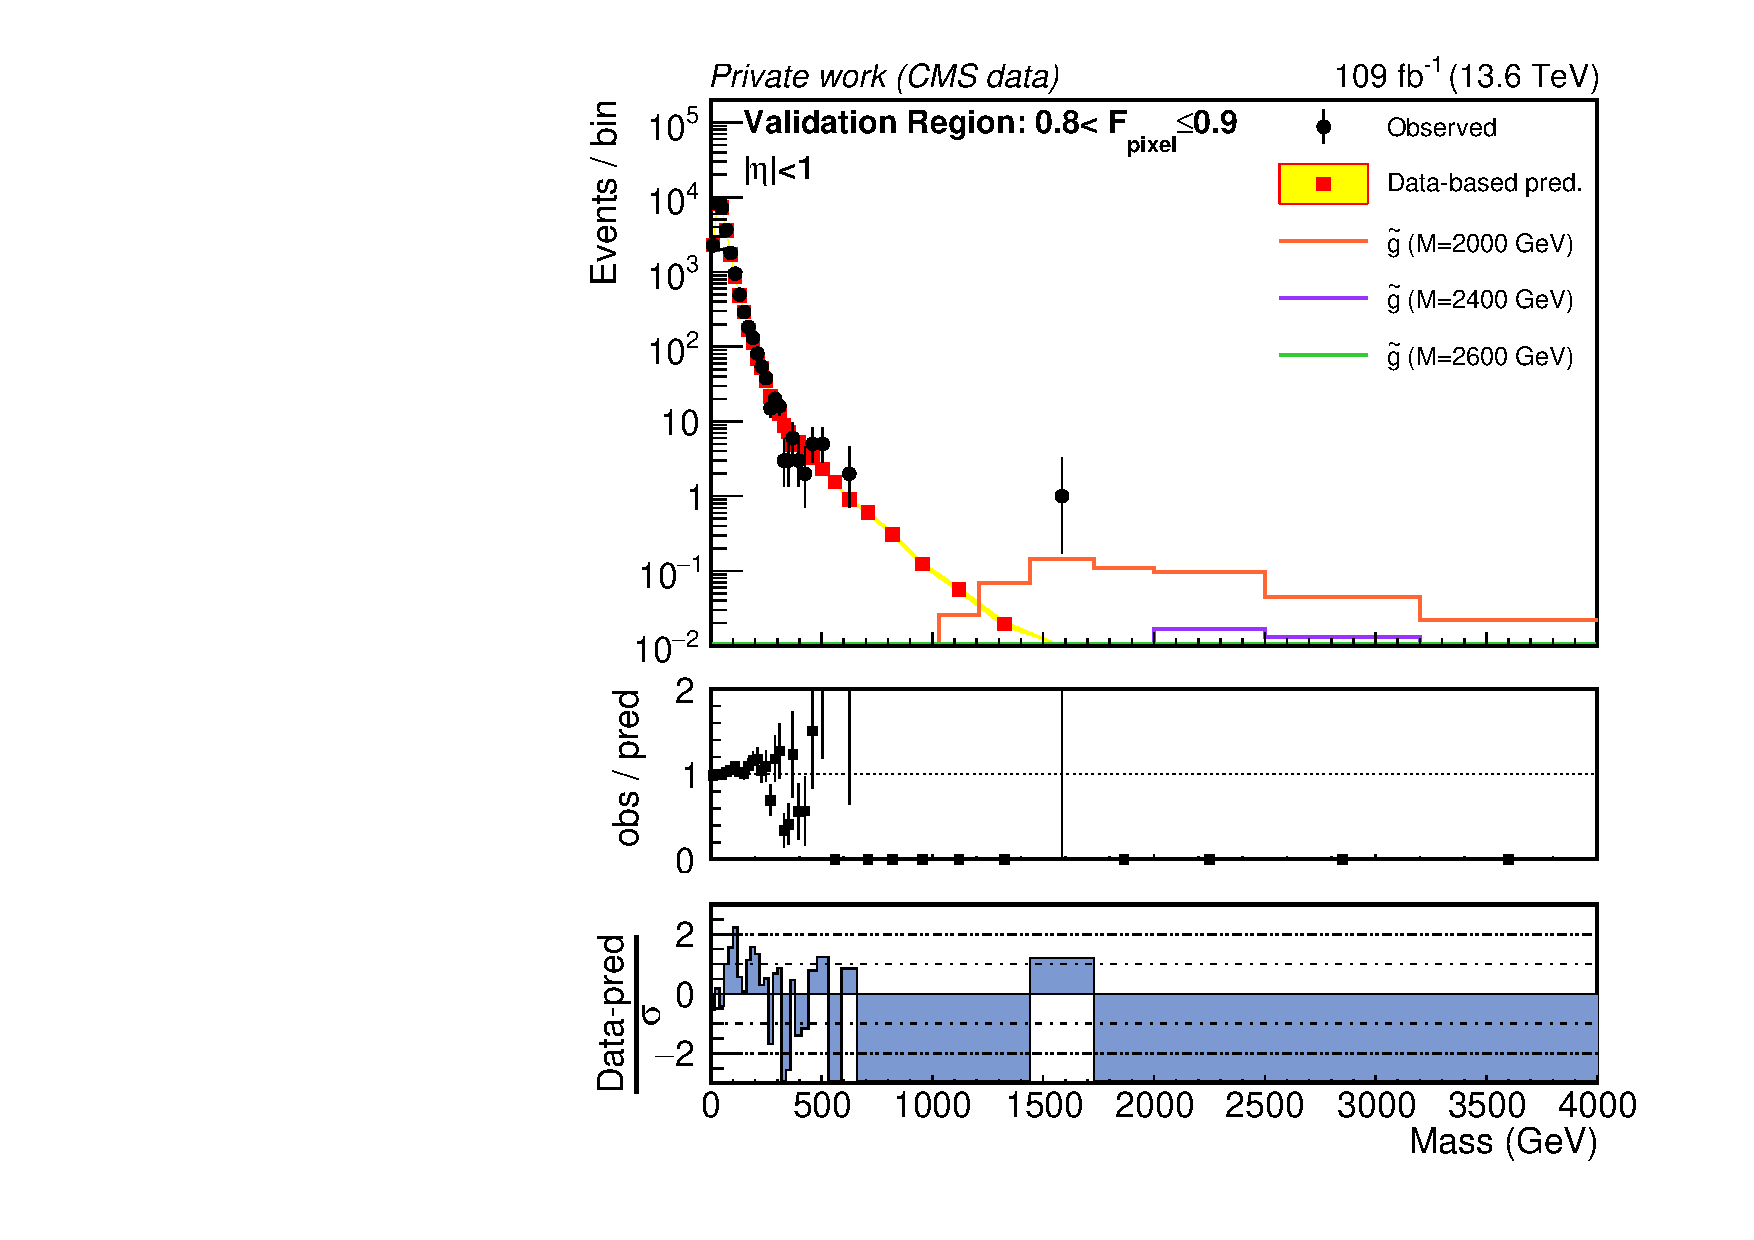
\includegraphics[width=0.49\linewidth,trim={1cm 0 1.2cm 0},clip]{Images/Ch4/mass_plot_Cnoabs_region8fp9_2024_onlyNominal_Eta1.pdf}
    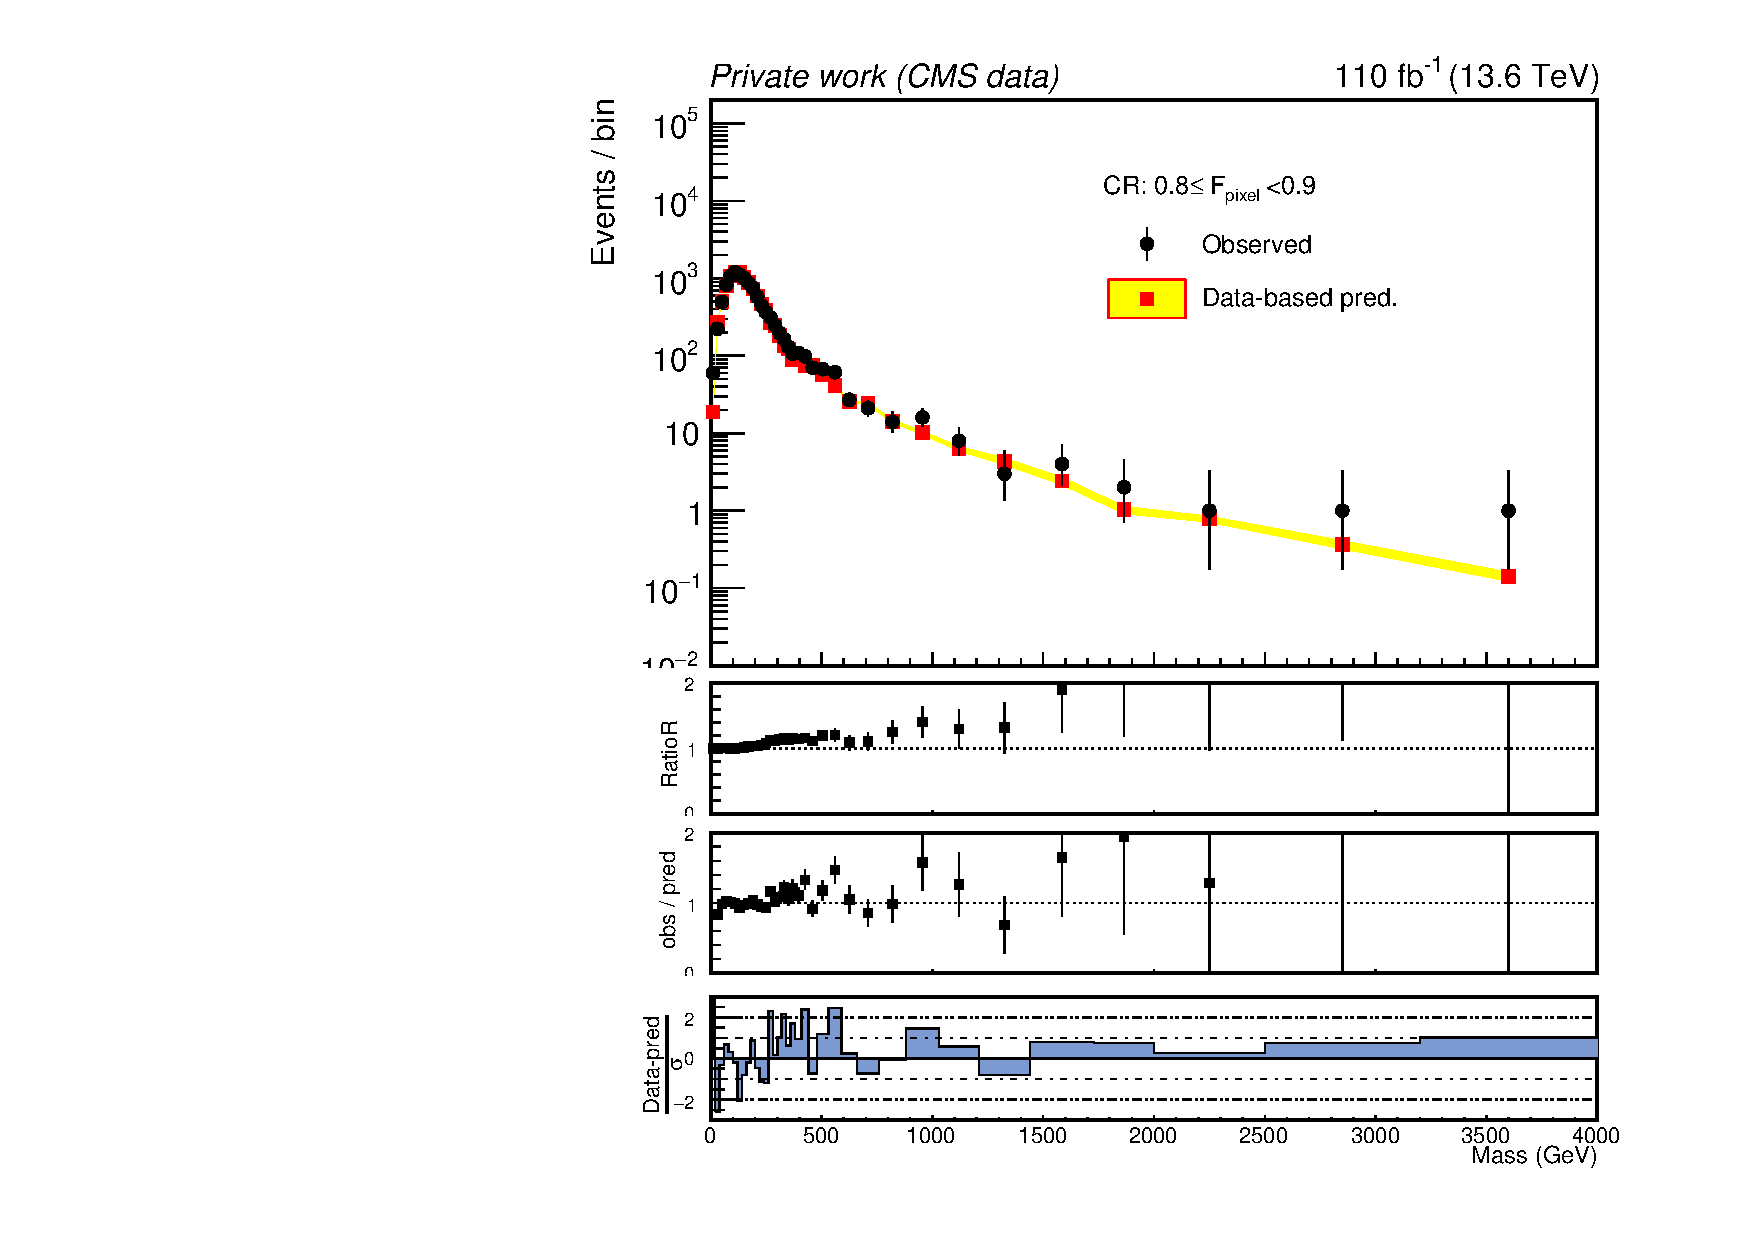
\includegraphics[width=0.49\linewidth,trim={1cm 0 1.2cm 0},clip]{Images/Ch4/mass_plot_Cnoabs_region8fp9_2024_onlyNominal_Eta1_2p4.pdf}
    \caption{Distribution de masse dans la région de validation pour les données de 2024, dans le tonneau $|\eta|<1$ (à gauche) et dans les bouchons $1\leq|\eta|<2{,}4$ (à droite). Les points noirs sont les données observées, les points rouges la prédiction avec son incertitude statistique (bande jaune). Plusieurs hypothèses de signal sont superposées. Les panneaux inférieurs présentent le rapport et l'écart normalisé (\textit{pull}) entre l'observation et la prédiction.}
    \label{fig:resume:vr}
\end{figure}

\subsection{Incertitudes systématiques}

Les incertitudes associées à la prédiction du bruit de fond sont obtenues en répétant la procédure avec des configurations modifiées : largeur des intervalles des gabarits en $\eta$, $I_h$ et $1/p$ doublée ou divisée par deux, paramètres d'ajustement des queues variés de $\pm1\sigma$, et correction de la faible corrélation résiduelle entre les gabarits et $F_\mathrm{pixel}$ omise. La variation du découpage en $1/p$ domine ; l'incertitude totale atteint environ 100\,\% dans les derniers intervalles de masse. Pour le signal, les sources considérées portent sur la luminosité (1,4\,\%), la modélisation de l'empilement, les SF de déclenchement, les paramètres $K_\mathrm{mass}$ et $C_\mathrm{mass}$ (écarts entre données et simulation), l'échelle d'énergie des jets et l'étalonnage des pixels (1,6\,\% sur l'efficacité de la coupure en $F_\mathrm{pixel}$, estimée à partir des conditions de fin 2024). Au voisinage du pic de signal, l'incertitude totale est de l'ordre de 10\,\%, dominée par l'empilement et les SF de déclenchement.

\subsection{Interprétation statistique}

La région de signal reste masquée (\textit{blind analysis}): seuls les événements de masse inférieure à 300~GeV ont été examinés, et ils sont en bon accord avec la prédiction. Les limites supérieures de la section efficace de production de paires de gluinos sont calculées à 95\,\% de niveau de confiance par la méthode CL$_\mathrm{s}$~\cite{CLSpaper}, avec une statistique de test fondée sur le rapport de vraisemblance profilé, dans l'approximation asymptotique~\cite{AsymptoticPaper} et à l'aide de l'outil \textsc{Combine}~\cite{CombinePaper} de la collaboration CMS. Les limites attendues sont obtenues à partir d'un jeu de données Asimov construit sous l'hypothèse de bruit de fond seul. Deux modèles statistiques sont comparés : une expérience de comptage dans une fenêtre de masse $[\mu_m-\sigma_m,\,\mu_m+2\sigma_m]$, adaptée à chaque hypothèse de signal, et un ajustement du spectre complet (analyse de forme) dans lequel la normalisation du bruit de fond est libre. Trois configurations en pseudo-rapidité sont étudiées : le tonneau seul ($|\eta|<1$), l'acceptance totale traitée comme un seul canal ($|\eta|<2{,}4$), et le tonneau et les bouchons ($1\leq|\eta|<2{,}4$) traités comme deux canaux distincts.

Le tonneau est pratiquement exempt de bruit de fond : pour $m_{\tilde{g}}=2000$~GeV, 12,7 événements de signal sont attendus dans la fenêtre de masse, contre 0,03 événement de bruit de fond, tandis que dans les bouchons, 4,6 événements de signal sont attendus pour 10 événements de bruit de fond. Par rapport à l'analyse du Run--2 restreinte au tonneau, le nombre d'événements de signal attendus est multiplié par un facteur allant de 1,5 à 1400~GeV jusqu'à 5,2 à 2600~GeV. Ce gain se répartit à parts comparables entre la hausse de la section efficace avec l'énergie (facteur de 1,4 à 2,4) et celle de l'efficacité de sélection (jusqu'à un facteur de 2), la luminosité n'y contribuant que pour 8\,\%.

Les masses exclues attendues sont présentées dans le \hyperref[tab:resume:limites]{Tableau~\ref*{tab:resume:limites}}, et les limites sont comparées sur la \hyperref[fig:resume:limites]{Figure~\ref*{fig:resume:limites}}. L'analyse de forme est toujours au moins aussi performante que le comptage. Traiter l'acceptance totale comme un seul canal dégrade la sensibilité, le bruit de fond des bouchons diluant la pureté du tonneau ; séparer les deux canaux permet au contraire à la vraisemblance de pondérer chaque région selon sa pureté, et la sensibilité est alors fixée par le tonneau. Dans la configuration la plus sensible, l'exclusion attendue atteint 2,42~TeV, soit plus de 300~GeV au-delà de la limite observée du Run--2 (2,08~TeV). Cette comparaison demande de la prudence : la limite du Run--2 est une limite observée, calculée avec la méthode CL$_\mathrm{s}$ complète et les sections efficaces à 13~TeV, alors que les limites présentées ici sont attendues et reposent sur l'approximation asymptotique, qui est optimiste lorsque le nombre d'événements attendus est très faible.

\vspace{0.5 cm}

\begin{table}[h!]
    \centering
    \small
    \renewcommand{\arraystretch}{1.3}
    \begin{tabular}{lcc}
        \toprule
        Configuration & Comptage & Analyse de forme \\
        \midrule
        Tonneau seul ($|\eta|<1$) & 2,39~TeV & 2,42~TeV \\
        Acceptance totale, un canal ($|\eta|<2{,}4$) & 2,15~TeV & 2,22~TeV \\
        Tonneau et bouchons séparés & 2,39~TeV & 2,42~TeV \\
        \bottomrule
    \end{tabular}
    \caption{Masses de gluino exclues attendues à 95\,\% de niveau de confiance, définies par l'intersection entre la limite médiane attendue et la section efficace théorique.}
    \label{tab:resume:limites}
\end{table}

\clearpage

La plus grande contribution individuelle d'un paramètre de nuisance à l'incertitude sur l'intensité du signal vaut environ 0,03 à 2000~GeV, pour une incertitude totale de ${}^{+0{,}28}_{-0{,}24}$ : la sensibilité est limitée par le nombre d'événements de signal, et non par les incertitudes systématiques.

\begin{figure}[h!]
    \centering
    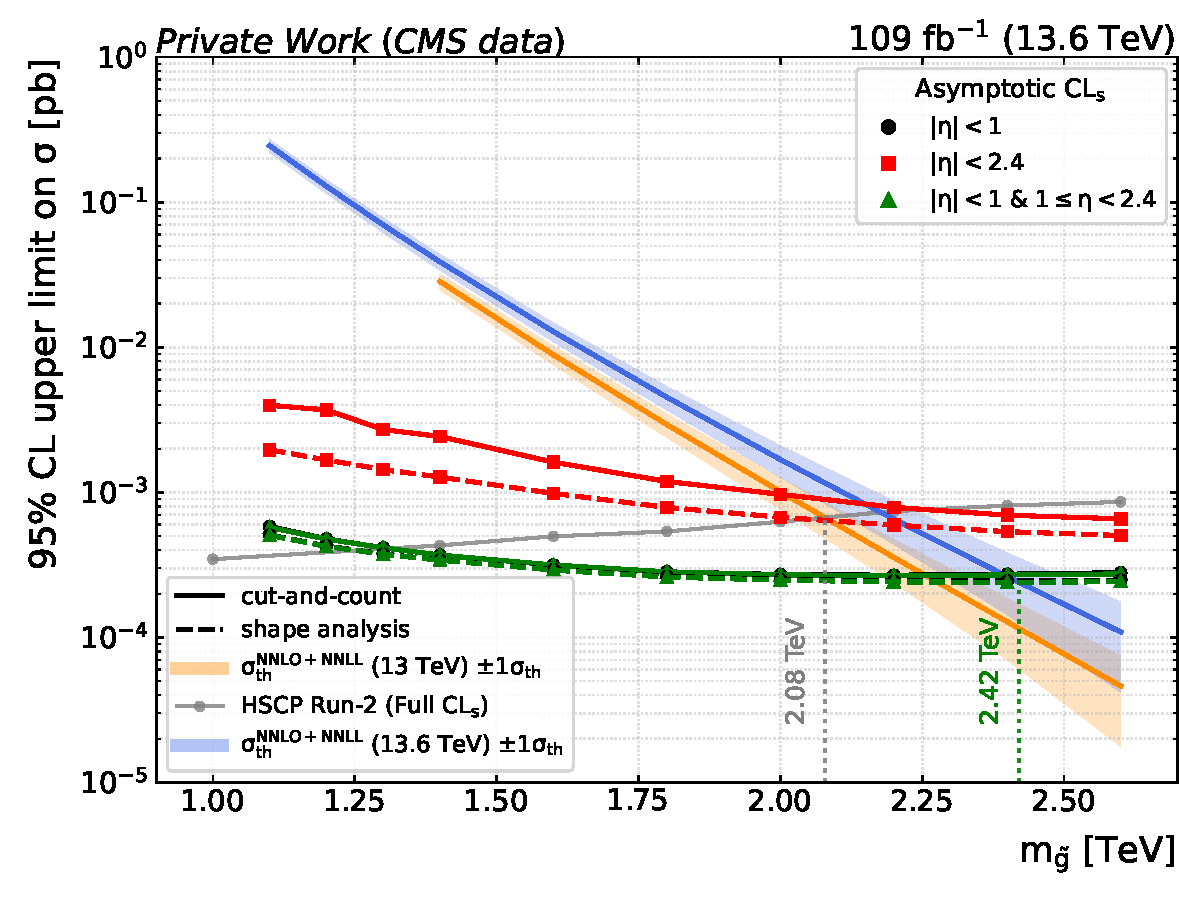
\includegraphics[width=0.72\linewidth]{Images/Ch4/ExpectedCompare_etaRebinPerso_Oldfit__PUppiMETcut_step5.pdf}
    \caption{Limites supérieures médianes attendues de la section efficace de production de paires de gluinos pour les trois configurations en pseudo-rapidité, avec la méthode de comptage (traits pleins) et l'analyse de forme (tirets). La limite observée de la recherche du Run--2~\cite{HSCP_Run2} est indiquée en gris, et les sections efficaces théoriques à 13 et 13,6~TeV sont représentées par les bandes orange et bleue.}
    \label{fig:resume:limites}
\end{figure}

\subsection{Perspectives}

Avant de lever le masquage de la région de signal, deux points restent à traiter : l'origine des événements de grande masse observés dans la région de validation des bouchons, et le calcul des limites finales avec la méthode CL$_\mathrm{s}$ complète, fondée sur des pseudo-expériences. Le résultat observé pourra alors être comparé à celui d'ATLAS (2,20~TeV).

La sensibilité étant limitée par le nombre d'événements, l'amélioration la plus importante viendra de l'ensemble des données du Run--3. La section efficace décroissant localement comme $e^{-m/m_0}$ avec $m_0\approx223$~GeV, la portée en masse augmente de $\Delta m\approx m_0\ln(\mathcal{L}'/\mathcal{L})$ : passer de 109 à 310~fb$^{-1}$ devrait porter l'exclusion attendue vers 2600--2700~GeV.

La même chaîne d'analyse s'applique directement aux $R$-hadrons de stops, et des interprétations pour des temps de vie finis ou pour des scénarios où les $R$-hadrons ne peuvent que perdre leur charge élargiraient l'espace des phases couvert.

Combiner les déclenchements sur la MET et sur les muons permettrait enfin de cibler également les HSCP de type leptonique.

À plus long terme, la jouvence du détecteur CMS pour la phase HL-LHC transformera cette recherche. La lecture binaire du trajectographe externe limitera les mesures de \dedx{} au trajectographe interne, soit au plus six mesures par trace contre une quinzaine aujourd'hui, et le temps de vol mesuré par le MTD deviendra la signature principale des particules lentes~\cite{CMS-DP-2022-025}.


%% ---------------------------------------------------------------------
\section*{Conclusion}
\addcontentsline{toc}{section}{Conclusion}
\label{sec:resume:conclusion}

Cette thèse présente une recherche de particules lourdes, stables et fortement ionisantes dans les données enregistrées par le détecteur CMS en 2024 à $\sqrt{s}=13{,}6$~TeV, en deux volets complémentaires.

Le premier traite de la saturation de l'électronique de lecture du trajectographe à pistes, qui biaise la mesure de \dedx{} précisément dans le régime visé par cette recherche. J'ai développé une correction fondée sur la forme des amas, qui distingue les amas en fonction de la position de la piste saturée et traite les cas d'une ou de deux pistes saturées consécutives. Validée par simulation et par les données de 2018, puis approuvée par les groupes de performance du trajectographe, elle a été utilisée pour les résultats publics de performance en \dedx{} issus des données de 2024 et 2025. Dans la recherche de HSCP, elle permet de retrouver la masse générée du signal, sans toutefois améliorer de façon mesurable les limites attendues, qui sont gouvernées par le nombre d'événements de signal. Son principal apport dépasse cette analyse : CMS dispose désormais d'une procédure de reconstruction des dépôts saturés, utilisable pour toute analyse reposant sur les mesures d'ionisation dans les pistes.

Le second volet est la recherche elle-même, que j'ai conçue presque entièrement. Les déclenchements sur la MET récupèrent des topologies de $R$-hadrons inaccessibles aux déclenchements sur les muons et portent l'efficacité de déclenchement des événements d'environ 11\,\% à 30\,\% pour $m_{\tilde{g}}=2000$~GeV, tandis que l'acceptance couvre désormais tout le trajectographe. Le bruit de fond, estimé à partir des données par une méthode ABCD utilisant pour la première fois $F_\mathrm{pixel}$, est validé dans une région dédiée. La région de signal restant masquée, les résultats sont présentés sous forme de limites attendues : en l'absence de signal, les gluinos seraient exclus jusqu'à 2,42~TeV à 95\,\% de niveau de confiance, soit plus de 300~GeV au-delà de l'exclusion observée du Run--2 à luminosité comparable. L'analyse de l'ensemble des données du Run--3 marquera l'aboutissement de la stratégie fondée sur l'ionisation, employée par CMS depuis le Run--1, et constituera le test le plus sensible de l'hypothèse de $R$-hadrons à long temps de vie avant l'arrivée des méthodes fondées sur le temps de vol dans le détecteur MTD au HL-LHC.

\addtocontents{toc}{\protect\setcounter{tocdepth}{3}}
\clearpage
\resumeLangueFin
\endgroup

% retour à la numérotation standard pour les chapitres suivants
\counterwithout*{figure}{section}
\counterwithout*{table}{section}
\counterwithout*{equation}{section}
\renewcommand{\thesection}{\thechapter.\arabic{section}}
\renewcommand{\thesubsection}{\thesection.\arabic{subsection}}
\setcounter{section}{0}
\setcounter{figure}{0}
\setcounter{table}{0}
\setcounter{equation}{0}
\adjustmtc